\documentclass[]{article}
\usepackage{lmodern}
\usepackage{amssymb,amsmath}
\usepackage{ifxetex,ifluatex}
\usepackage{fixltx2e} % provides \textsubscript
\ifnum 0\ifxetex 1\fi\ifluatex 1\fi=0 % if pdftex
  \usepackage[T1]{fontenc}
  \usepackage[utf8]{inputenc}
\else % if luatex or xelatex
  \ifxetex
    \usepackage{mathspec}
  \else
    \usepackage{fontspec}
  \fi
  \defaultfontfeatures{Ligatures=TeX,Scale=MatchLowercase}
\fi
% use upquote if available, for straight quotes in verbatim environments
\IfFileExists{upquote.sty}{\usepackage{upquote}}{}
% use microtype if available
\IfFileExists{microtype.sty}{%
\usepackage{microtype}
\UseMicrotypeSet[protrusion]{basicmath} % disable protrusion for tt fonts
}{}
\usepackage[margin=1in]{geometry}
\usepackage{hyperref}
\hypersetup{unicode=true,
            pdftitle={Tutorial on Bayesian Statistics.   Homework from BDA3},
            pdfauthor={Fernando Hoces de la Guardia; Guided by: Susan Paddock},
            pdfborder={0 0 0},
            breaklinks=true}
\urlstyle{same}  % don't use monospace font for urls
\usepackage{color}
\usepackage{fancyvrb}
\newcommand{\VerbBar}{|}
\newcommand{\VERB}{\Verb[commandchars=\\\{\}]}
\DefineVerbatimEnvironment{Highlighting}{Verbatim}{commandchars=\\\{\}}
% Add ',fontsize=\small' for more characters per line
\usepackage{framed}
\definecolor{shadecolor}{RGB}{248,248,248}
\newenvironment{Shaded}{\begin{snugshade}}{\end{snugshade}}
\newcommand{\KeywordTok}[1]{\textcolor[rgb]{0.13,0.29,0.53}{\textbf{#1}}}
\newcommand{\DataTypeTok}[1]{\textcolor[rgb]{0.13,0.29,0.53}{#1}}
\newcommand{\DecValTok}[1]{\textcolor[rgb]{0.00,0.00,0.81}{#1}}
\newcommand{\BaseNTok}[1]{\textcolor[rgb]{0.00,0.00,0.81}{#1}}
\newcommand{\FloatTok}[1]{\textcolor[rgb]{0.00,0.00,0.81}{#1}}
\newcommand{\ConstantTok}[1]{\textcolor[rgb]{0.00,0.00,0.00}{#1}}
\newcommand{\CharTok}[1]{\textcolor[rgb]{0.31,0.60,0.02}{#1}}
\newcommand{\SpecialCharTok}[1]{\textcolor[rgb]{0.00,0.00,0.00}{#1}}
\newcommand{\StringTok}[1]{\textcolor[rgb]{0.31,0.60,0.02}{#1}}
\newcommand{\VerbatimStringTok}[1]{\textcolor[rgb]{0.31,0.60,0.02}{#1}}
\newcommand{\SpecialStringTok}[1]{\textcolor[rgb]{0.31,0.60,0.02}{#1}}
\newcommand{\ImportTok}[1]{#1}
\newcommand{\CommentTok}[1]{\textcolor[rgb]{0.56,0.35,0.01}{\textit{#1}}}
\newcommand{\DocumentationTok}[1]{\textcolor[rgb]{0.56,0.35,0.01}{\textbf{\textit{#1}}}}
\newcommand{\AnnotationTok}[1]{\textcolor[rgb]{0.56,0.35,0.01}{\textbf{\textit{#1}}}}
\newcommand{\CommentVarTok}[1]{\textcolor[rgb]{0.56,0.35,0.01}{\textbf{\textit{#1}}}}
\newcommand{\OtherTok}[1]{\textcolor[rgb]{0.56,0.35,0.01}{#1}}
\newcommand{\FunctionTok}[1]{\textcolor[rgb]{0.00,0.00,0.00}{#1}}
\newcommand{\VariableTok}[1]{\textcolor[rgb]{0.00,0.00,0.00}{#1}}
\newcommand{\ControlFlowTok}[1]{\textcolor[rgb]{0.13,0.29,0.53}{\textbf{#1}}}
\newcommand{\OperatorTok}[1]{\textcolor[rgb]{0.81,0.36,0.00}{\textbf{#1}}}
\newcommand{\BuiltInTok}[1]{#1}
\newcommand{\ExtensionTok}[1]{#1}
\newcommand{\PreprocessorTok}[1]{\textcolor[rgb]{0.56,0.35,0.01}{\textit{#1}}}
\newcommand{\AttributeTok}[1]{\textcolor[rgb]{0.77,0.63,0.00}{#1}}
\newcommand{\RegionMarkerTok}[1]{#1}
\newcommand{\InformationTok}[1]{\textcolor[rgb]{0.56,0.35,0.01}{\textbf{\textit{#1}}}}
\newcommand{\WarningTok}[1]{\textcolor[rgb]{0.56,0.35,0.01}{\textbf{\textit{#1}}}}
\newcommand{\AlertTok}[1]{\textcolor[rgb]{0.94,0.16,0.16}{#1}}
\newcommand{\ErrorTok}[1]{\textcolor[rgb]{0.64,0.00,0.00}{\textbf{#1}}}
\newcommand{\NormalTok}[1]{#1}
\usepackage{longtable,booktabs}
\usepackage{graphicx,grffile}
\makeatletter
\def\maxwidth{\ifdim\Gin@nat@width>\linewidth\linewidth\else\Gin@nat@width\fi}
\def\maxheight{\ifdim\Gin@nat@height>\textheight\textheight\else\Gin@nat@height\fi}
\makeatother
% Scale images if necessary, so that they will not overflow the page
% margins by default, and it is still possible to overwrite the defaults
% using explicit options in \includegraphics[width, height, ...]{}
\setkeys{Gin}{width=\maxwidth,height=\maxheight,keepaspectratio}
\IfFileExists{parskip.sty}{%
\usepackage{parskip}
}{% else
\setlength{\parindent}{0pt}
\setlength{\parskip}{6pt plus 2pt minus 1pt}
}
\setlength{\emergencystretch}{3em}  % prevent overfull lines
\providecommand{\tightlist}{%
  \setlength{\itemsep}{0pt}\setlength{\parskip}{0pt}}
\setcounter{secnumdepth}{0}
% Redefines (sub)paragraphs to behave more like sections
\ifx\paragraph\undefined\else
\let\oldparagraph\paragraph
\renewcommand{\paragraph}[1]{\oldparagraph{#1}\mbox{}}
\fi
\ifx\subparagraph\undefined\else
\let\oldsubparagraph\subparagraph
\renewcommand{\subparagraph}[1]{\oldsubparagraph{#1}\mbox{}}
\fi

%%% Use protect on footnotes to avoid problems with footnotes in titles
\let\rmarkdownfootnote\footnote%
\def\footnote{\protect\rmarkdownfootnote}

%%% Change title format to be more compact
\usepackage{titling}

% Create subtitle command for use in maketitle
\newcommand{\subtitle}[1]{
  \posttitle{
    \begin{center}\large#1\end{center}
    }
}

\setlength{\droptitle}{-2em}

  \title{Tutorial on Bayesian Statistics. Homework from BDA3}
    \pretitle{\vspace{\droptitle}\centering\huge}
  \posttitle{\par}
    \author{Fernando Hoces de la Guardia \\ Guided by: Susan Paddock}
    \preauthor{\centering\large\emph}
  \postauthor{\par}
    \date{}
    \predate{}\postdate{}
  

\begin{document}
\maketitle

\section{Chapter 1}\label{chapter-1}

\subsection{1.1}\label{section}

\subsubsection{1a:}\label{a}

\[
\begin{aligned}
p(y)  &= \frac{1}{2} \left( p(y| \theta = 1) + p(y| \theta = 2) \right) \nonumber\\
      &= \frac{1}{2} \left( N(y|1,2^{2}) + N(y|2,2^{2}) \right)
\end{aligned}
\]

\begin{Shaded}
\begin{Highlighting}[]
\NormalTok{domain          <-}\StringTok{ }\KeywordTok{seq}\NormalTok{(}\OperatorTok{-}\DecValTok{7}\NormalTok{,}\DecValTok{10}\NormalTok{,.}\DecValTok{02}\NormalTok{)}
\NormalTok{dens            <-}\StringTok{ }\FloatTok{0.5}\OperatorTok{*}\KeywordTok{dnorm}\NormalTok{(domain,}\DecValTok{1}\NormalTok{,}\DecValTok{2}\NormalTok{) }\OperatorTok{+}\StringTok{ }\FloatTok{0.5}\OperatorTok{*}\KeywordTok{dnorm}\NormalTok{(domain,}\DecValTok{2}\NormalTok{,}\DecValTok{2}\NormalTok{)}
\KeywordTok{plot}\NormalTok{ (domain, dens, }\DataTypeTok{ylim=}\KeywordTok{c}\NormalTok{(}\DecValTok{0}\NormalTok{,}\FloatTok{1.1}\OperatorTok{*}\KeywordTok{max}\NormalTok{(dens)),}
\DataTypeTok{type=}\StringTok{"l"}\NormalTok{, }\DataTypeTok{xlab=}\StringTok{"y"}\NormalTok{, }\DataTypeTok{ylab=}\StringTok{""}\NormalTok{, }\DataTypeTok{xaxs=}\StringTok{"i"}\NormalTok{,}
\DataTypeTok{yaxs=}\StringTok{"i"}\NormalTok{, }\DataTypeTok{yaxt=}\StringTok{"n"}\NormalTok{, }\DataTypeTok{bty=}\StringTok{"n"}\NormalTok{, }\DataTypeTok{cex=}\DecValTok{2}\NormalTok{)}
\end{Highlighting}
\end{Shaded}

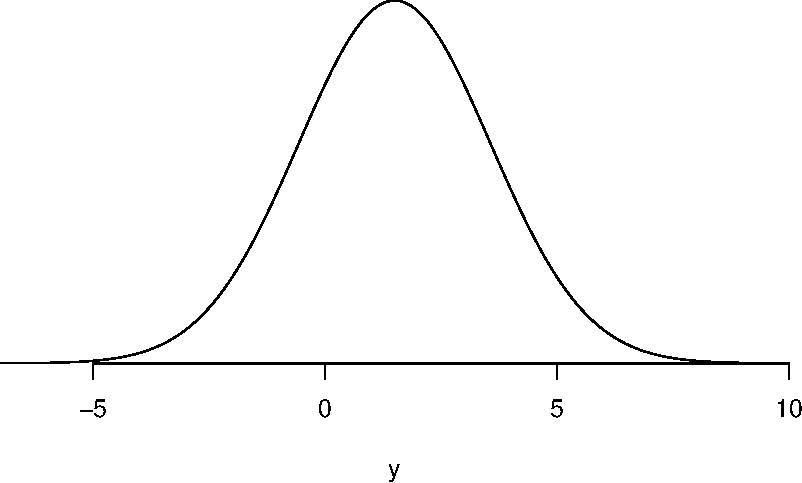
\includegraphics{Untitled_files/figure-latex/unnamed-chunk-1-1.pdf}

\subsubsection{1b:}\label{b}

\[
\begin{aligned}
p(\theta = 1 | y = 1 ) &= \frac{p(\theta = 1)p(y = 1| \theta = 1)}{\sum_{i=1}^{2}p(\theta = i)p(y = 1| \theta = i)} \nonumber \\
                      &= \frac{0.5N(1|1,4)}{\sum_{i=1}^{2}0.5N(1|i,4)}
\end{aligned}
\]

\begin{Shaded}
\begin{Highlighting}[]
\NormalTok{p.theta.}\DecValTok{1}\NormalTok{       <-}\StringTok{ }\ControlFlowTok{function}\NormalTok{(sigma) \{}
\NormalTok{  res1          <-}\StringTok{ }\NormalTok{(}\FloatTok{0.5}\OperatorTok{*}\KeywordTok{dnorm}\NormalTok{(}\DecValTok{1}\NormalTok{,}\DecValTok{1}\NormalTok{,sigma)) }\OperatorTok{/}\NormalTok{(}\KeywordTok{sum}\NormalTok{(}\FloatTok{0.5}\OperatorTok{*}\KeywordTok{dnorm}\NormalTok{(}\DecValTok{1}\NormalTok{,}\KeywordTok{c}\NormalTok{(}\DecValTok{1}\NormalTok{,}\DecValTok{2}\NormalTok{),sigma)))}
  \KeywordTok{return}\NormalTok{(res1)}
\NormalTok{  \}}
\end{Highlighting}
\end{Shaded}

Evaluating the last expression in the respective cumulative distribution
function we get:0.5312094. \textbf{Note: even though we are adding
``discrete'' number of probabilities, we are still in the continuous
space (but for \(y=1\)) and should evaluate the probabilities in the
density function.}

\subsubsection{1c:}\label{c}

\textbf{Table 1: Posterior probabilty of \(\theta = 1\), af a function
of \(\sigma\)}

\begin{longtable}[]{@{}rc@{}}
\toprule
\(\sigma\) & \$p(\theta = 1\tabularnewline
\midrule
\endhead
0.25 & 0.9996646\tabularnewline
0.5 & 0.8807971\tabularnewline
1 & 0.6224593\tabularnewline
2 & 0.5312094\tabularnewline
4 & 0.5078119\tabularnewline
8 & 0.5019531\tabularnewline
\bottomrule
\end{longtable}

\subsubsection{\texorpdfstring{1.3
\textbf{{[}NEW{]}}}{1.3 {[}NEW{]}}}\label{new}

First: compute posterior of probability of having \(Xx\) genes knowing
that parents have brown eyes and individual has brown eyes:

\[
\begin{aligned}
&p(Xx | \text{Person and parents have brown eyes}) = \\
&\frac{ Pr(Xx|(XX,XX))Pr((XX,XX)) + Pr(Xx|(Xx,XX))Pr((Xx,XX)) + Pr(Xx|(Xx,Xx))Pr((Xx,Xx)) }
{Pr(Brown|(XX,XX))Pr((XX,XX)) + Pr(Brown|(Xx,XX))Pr((Xx,XX)) + Pr(Brown|(Xx,Xx))Pr((Xx,Xx)) } \nonumber  \\
&=       \frac{ 0 \cdot (1-p)^{4} + 1/2 \cdot 4p(1-p)^{3} + 1/2 \cdot 4p(1-p)^{2} }
{ 1 \cdot (1-p)^{4} + 1 \cdot 4p(1-p)^{3} + (1-Pr(Blue|(Xx,Xx))) \cdot 4p(1-p)^{2} } \\
&=       \frac{ 0 \cdot (1-p)^{4} + 1/2 \cdot 4p(1-p)^{3} + 1/2 \cdot 4p(1-p)^{2} }
{ 1 \cdot (1-p)^{4} + 1 \cdot 4p(1-p)^{3} + 3/4 \cdot 4p(1-p)^{2} } \\
&= \frac{2p}{1+2p}
\end{aligned}
\]

This posterior (\(p(Xx | \text{Person and parents have brown eyes})\))
will be the new prior when computing the probability that Judy's is
\(Xx\) given that all her kids are brown eyed (husband is \(Xx\)). \[
\begin{aligned}
&p(Judy = Xx | \text{all n kids brown eyes (AKBE) + previous info.}) = \nonumber \\
&\frac{P(Judy = Xx) P(AKBE|Judy=Xx) }{P(Judy = Xx) P(AKBE|Judy=Xx) + P(Judy \neq  Xx) P(AKBE|Judy \neq Xx)} \\
&= \frac{ \frac{2p}{1+2p} (\frac{3}{4})^{n} }{ \frac{2p}{1+2p} (\frac{3}{4})^{n} + \frac{1}{1+2p} }
\end{aligned}
\]

Now we want to compute the probability that the first grandchildren will
have blue eyes. We know that all Judy's children have brown eyes, hence
have genes \(Xx\) or \(XX\). It follows that the grandkids will have
blue eyes only if the kids have \(Xx\) genes. A kid will have \(Xx\) if
Judy has \(Xx\) and she and her husband provide \(Xx\) (\(pr=2/3\),
remember that the kid has brown eyes) or if she has \(XX\) and her
husband provide \(Xx\) (\(pr=1/2\)). Hence the probability of any kid to
be \(Xx\) is: \[
\begin{aligned}
P(kid = Xx| \text{all info}) &= P(kid = Xx| \text{all info} + Judy = Xx)P(Judy = Xx) + \\  &P(kid = Xx| \text{all info} + Judy \neq Xx)P(Judy \neq Xx) \nonumber \\
&= \left( \frac{2}{3} \right) \frac{ \frac{2p}{1+2p} (\frac{3}{4})^{n} }{ \frac{2p}{1+2p} (\frac{3}{4})^{n} + \frac{1}{1+2p} } + \left( \frac{1}{2} \right) \frac{ \frac{1}{1+2p} (\frac{3}{4})^{n} }{ \frac{2p}{1+2p} (\frac{3}{4})^{n} + \frac{1}{1+2p} }
\end{aligned}
\]

Conditional on a kid having \(Xx\) the probability of having a
grandchild with blue eyes is 0,1/4 and 1/2 if the spouse is \(XX\),
\(Xx\) and \(xx\) respectively. Each spouse type has a probability of
\((1-p)^{2}, 2p(1-p)\) and \(p^2\) respectively. Hence, the probability
of a grandkid with blue eyes is: \[
\begin{aligned}
P(Grandchildren = Blue|\text{all info}) &=  \frac{ \frac{2}{3}\frac{2p}{1+2p} + \frac{1}{2}\frac{1}{1+2p} }{\frac{2p}{1+2p} (\frac{3}{4})^{n} + \frac{1}{1+2p} } \left( \frac{1}{4}2p(1-p) + \frac{1}{2}p^{2} \right) \\ 
&= \frac{ \frac{2}{3}\frac{2p}{1+2p} + \frac{1}{2}\frac{1}{1+2p} }{\frac{2p}{1+2p} (\frac{3}{4})^{n} + \frac{1}{1+2p} } \left( \frac{1}{2}p \right) \nonumber
\end{aligned}
\] Note: This solution was reverse engineered from
\href{http://www.stat.columbia.edu/~gelman/book/solutions3.pdf}{here.}.
A few additional lines were added.

\subsection{\texorpdfstring{1.6
\textbf{{[}NEW{]}}}{1.6 {[}NEW{]}}}\label{new-1}

The trick here is that the probability of having a fraternal twin birth
with two boys is \(1/4 \times 1/125\) and a identical twin birth of boys
is \(1/2 \times 1/300\). Hence the probability that Elvis had an
identical twin is \(5/11\).

\subsection{\texorpdfstring{1.7 \emph{Let's Make a
Deal}}{1.7 Let's Make a Deal}}\label{lets-make-a-deal}

Calculate the probability of winning for each box after one of the empty
boxes has been revealed and is not a winning box.

Lets define the following events:\\
* \(A:\) The participant chose the right box at the beginning.\\
* \(B:\) The host opens a particular box, among the unchosen ones, such
that is empty.\\
* \(C:\) Among the unchosen boxes the host chooses a empty box.

And let's compute the probabilities of each of this events.\\
\[
\begin{aligned}
Pr(A) &= 1/3\\
Pr(C) &= 1/2\\
Pr(B) &= Pr(B|A)Pr(A) + Pr(B|\neg A)Pr(\neg A) = (1/2)*(1/3) + Pr(B|\neg A)*(2/3)\\
      &= 1/6 + 2/3*(Pr(B|\neg A,C)Pr(C) + Pr(B|\neg A,\neg C)Pr(\neg C)) \\
      &= 1/6 + 2/3*(1*(1/2) + 0*(1/2)) = 1/2 
\end{aligned}  
\] Using Bayes' theorem we have that the probability of choosing the
right box from the beginning, conditional on a unchosen box being
revealed as a losing one is:

\[ Pr(A|B) = \frac{Pr(A)Pr(B|A)}{Pr(B)} = \frac{(1/3)*(1/2)}{1/2}=\frac{1}{3}\]

The participant's chances are not equal across remaining boxes! She is
worst of staying with her original choice (33\% probability of wining
instead of 50\%!).

More generally if there were \(n\) boxes in total and \(i\) boxes where
revealed, we have that the wrong way of updating the probabilities
(\(1/(n-i)\)) and the Bayesian update
(\(\frac{i+n*(n-1-i)}{n*(n-i)*(n-i-1)}\)) differ significantly as
\(i \rightarrow n\). For example the following graph plots both
probabilities of winning in a contest with 50 boxes as the host opens
\(i\) boxes.

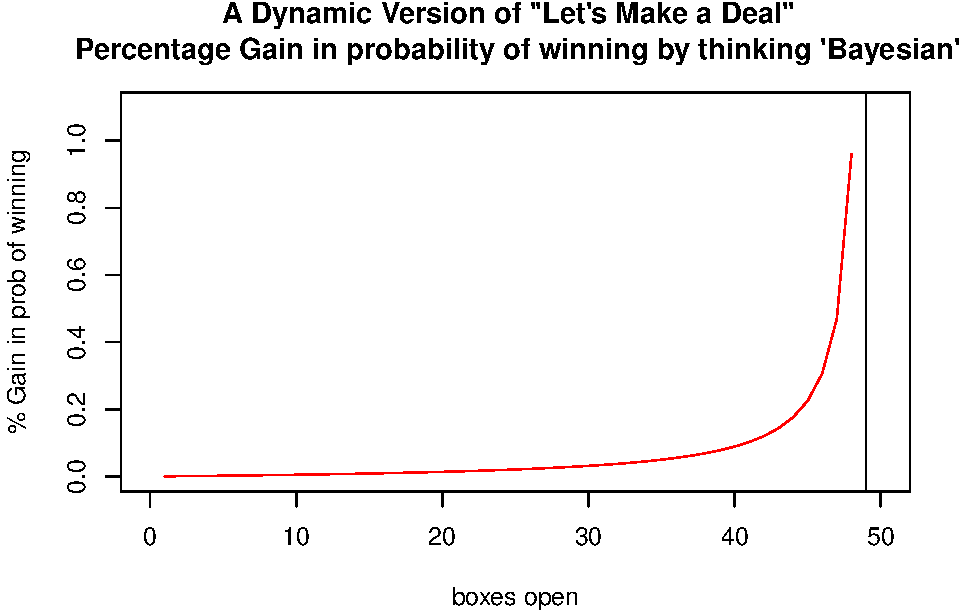
\includegraphics{Untitled_files/figure-latex/unnamed-chunk-4-1.pdf}
Looking at the graph it seems that the advantages of thinking in a
Bayesian fashion are certainly parameter-specific. Also notice that the
player here chooses a ``stubborn'' strategy, I suspect that if she
changes boxes in a optimal way the improvement in her chances will be
slightly less. Maybe that is the reason why we don't think in a Bayesian
fashion all the time.

\section{Chapter 2}\label{chapter-2}

\subsection{2.1}\label{section-1}

\[
\begin{aligned}
P(\theta) &= Beta(4,4)  \\
P( y | \theta) &= Bin(y|n,\theta)  \\
\Rightarrow P(\theta|y) &= Beta(4+y,4+(n-y))
\end{aligned}
\]\\
The \textbf{wrong} way to answer the question would be:\\
\[
\begin{aligned}
P(\theta|y<3) &\propto \sum_{i=0}^{2}Beta(4+i,4+(n-i))
\end{aligned}
\] The \textbf{right} way to answer the question would be:\\
\[
\begin{aligned}
P( y<3 | \theta) &= \sum_{i=0}^{2}Bin(i|n,\theta)\\
\Rightarrow P(\theta|y) &\propto \sum_{i=0}^{2} {n \choose i} Beta(4+i,4+(n-i))\\  
\end{aligned}
\] In this case some part of the proportionality constant \emph{does}
matter.

\begin{Shaded}
\begin{Highlighting}[]
\NormalTok{domain <-}\StringTok{ }\KeywordTok{seq}\NormalTok{(}\DecValTok{0}\NormalTok{,}\DecValTok{1}\NormalTok{,.}\DecValTok{01}\NormalTok{)}
\NormalTok{dens =}\StringTok{ }\KeywordTok{apply}\NormalTok{(}\KeywordTok{sapply}\NormalTok{(}\DecValTok{0}\OperatorTok{:}\DecValTok{2}\NormalTok{,}\ControlFlowTok{function}\NormalTok{(x) }\KeywordTok{choose}\NormalTok{(}\DecValTok{10}\NormalTok{,x)}\OperatorTok{*}\KeywordTok{dbeta}\NormalTok{(domain,}\DecValTok{4}\OperatorTok{+}\NormalTok{x,}\DecValTok{4}\OperatorTok{+}\DecValTok{10}\OperatorTok{-}\NormalTok{x)),}\DecValTok{1}\NormalTok{,sum)}
\KeywordTok{plot}\NormalTok{(domain, dens, }\DataTypeTok{type=}\StringTok{"l"}\NormalTok{)}
\end{Highlighting}
\end{Shaded}

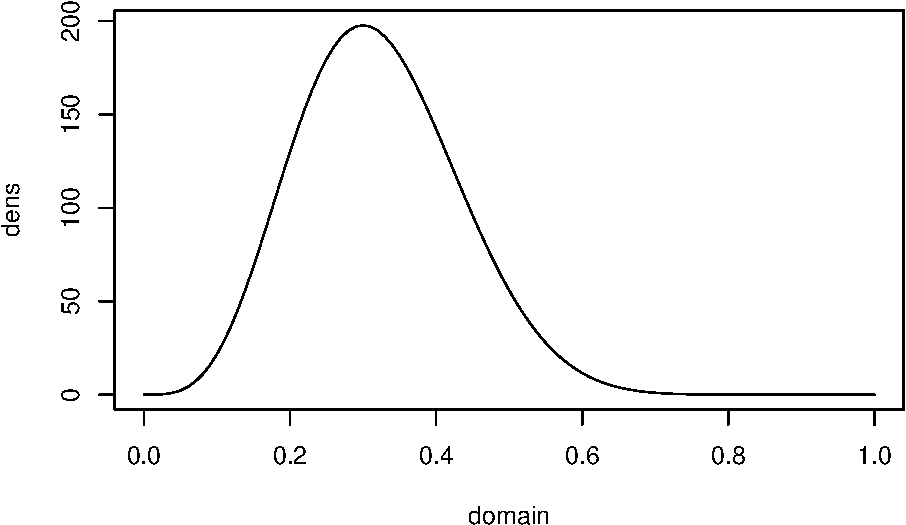
\includegraphics{Untitled_files/figure-latex/unnamed-chunk-5-1.pdf}

\subsection{2.14}\label{section-2}

\subsubsection{2.14a}\label{a-1}

Deriving the posterior for a normal likelihood with known variance,
unknown mean, and using a normal prior.
\href{http://www.people.fas.harvard.edu/~plam/teaching/methods/conjugacy/conjugacy_print.pdf}{Slide
15 here}

\textbf{Note:} a good reminder of the main conjugacy relationships can
be found
\href{http://www.johndcook.com/conjugate_prior_diagram.html}{here}

\subsubsection{\texorpdfstring{2.16a
\textbf{{[}NEW{]}}}{2.16a {[}NEW{]}}}\label{a-new}

Suppose \(y \sim Bin(n,\theta)\), with
\(\theta \sim Beta(\alpha, \beta)\). Derive marginal distribution of
\(y\) (unconditional on \(\theta\))

\[
\begin{aligned}
P(y = k) &= \int_{O}^{1}  p(y,\theta) d\theta \\
 &= \int_{O}^{1}  p(y|\theta) p(\theta) d\theta \\
 &= \int_{O}^{1}   {n \choose k} \theta^{k} ( 1 - \theta)^{n-k} \times 
 \frac{\Gamma(\alpha + \beta)}{\Gamma(\alpha)\Gamma(\beta)} \theta^{\alpha - 1} ( 1 - \theta)^{\beta - 1} d\theta \\
 &= {n \choose k} \frac{\Gamma(\alpha + \beta)}{\Gamma(\alpha)\Gamma(\beta)} \int_{O}^{1}  \theta^{k + \alpha - 1} ( 1 - \theta)^{n - k + \beta - 1} d\theta \\
 &= {n \choose k} \frac{\Gamma(\alpha + \beta)}{\Gamma(\alpha)\Gamma(\beta)} \int_{O}^{1} \frac{\Gamma(\alpha + k)\Gamma(\beta + n - k)}{\Gamma(\alpha + \beta + n)} \frac{\Gamma(\alpha + \beta + n)}{\Gamma(\alpha + k)\Gamma(\beta + n - k)}   \theta^{k + \alpha - 1} ( 1 - \theta)^{n - k + \beta - 1} d\theta \\
 &= {n \choose k} \frac{\Gamma(\alpha + \beta)}{\Gamma(\alpha)\Gamma(\beta)} \frac{\Gamma(\alpha + k)\Gamma(\beta + n - k)}{\Gamma(\alpha + \beta + n)}  \int_{O}^{1}  \frac{\Gamma(\alpha + \beta + n)}{\Gamma(\alpha + k)\Gamma(\beta + n - k)}   \theta^{k + \alpha - 1} ( 1 - \theta)^{n - k + \beta - 1} d\theta \\
 &= {n \choose k} \frac{\Gamma(\alpha + \beta)}{\Gamma(\alpha)\Gamma(\beta)} \frac{\Gamma(\alpha + k)\Gamma(\beta + n - k)}{\Gamma(\alpha + \beta + n)} 
\end{aligned}
\]

Where the second to last line follows from integrating the density of a
\(Beta(k + \alpha, n - k + \beta)\)

\subsection{\texorpdfstring{2.19 \textbf{{[}NEW{]}} Exponential model
with conjugate prior
distribution:}{2.19 {[}NEW{]} Exponential model with conjugate prior distribution:}}\label{new-exponential-model-with-conjugate-prior-distribution}

\subsubsection{2.19a}\label{a-2}

Prove conyugacy for \(y_{i}|\theta \sim Exp(\theta)\) for
\(i= 1, \dots ,n\) , iid, and \(\theta \sim Gamma(\alpha, \beta)\).

\[
\begin{aligned}
p(\theta| \mathbf{y}) &\propto p(\mathbf{y}|\theta)p(\theta) \\
&= p(\theta) \prod_{i=1}^{n} p(y_{i}|\theta) \\
&= \frac{\beta^{\alpha}}{\Gamma(\alpha)} \theta^{\alpha - 1} exp(-\beta \theta) \times \prod_{i=1}^{n} \theta exp(-\theta y_{i}) \\
&= \frac{\beta^{\alpha}}{\Gamma(\alpha)} \theta^{\alpha - 1} exp(-\beta \theta) \times \prod_{i=1}^{n} \theta exp(-\theta y_{i}) \\
&= \frac{\beta^{\alpha}}{\Gamma(\alpha)}  \times  \theta^{\alpha + n - 1} exp(-\theta(\beta + \sum y_{i}) ) \\
&\propto \frac{(\beta + \sum y_{i})^{\alpha + n}}{\Gamma(\alpha + n)} \theta^{\alpha + n - 1} exp(-\theta(\beta + \sum y_{i}) ) \\
&= Gamma(\alpha + n, \beta + \sum y_{i}) 
\end{aligned} 
\]

\subsubsection{2.19b}\label{b-1}

Show that the equivalent prior specification for the mean
\(\phi = 1/\theta\), is inverse-gamma.\\
\textbf{Solution:} We will use the transformation method. For this
purpose we define: \(\phi = g(\theta) = 1/\theta\), This implies that
\(g^{-1}(\phi) = 1/\phi\) and
\(\frac{d}{d\phi} g^{-1}(\phi) = - 1/\phi^{2}\). Now:

\[
\begin{aligned}
f_{\phi}(\phi) &= f_{\theta}\left( g^{-1}(\phi) \right) |\frac{d}{d\phi}g^{-1}(\phi)|\\
&= \frac{\beta^{\alpha}}{\Gamma(\alpha)} \frac{1}{\phi^{(\alpha - 1)}}  exp(-\beta/\phi) \frac{1}{\phi^2} \\
&= \frac{\beta^{\alpha}}{\Gamma(\alpha)} \phi^{- (\alpha + 1)}  exp(-\beta/\phi) \\
&= Inv\text{-}Gamma(\phi)
\end{aligned}
\]

\subsubsection{2.19c}\label{c-1}

The length of life (\(y_{i}\)) of a ligth bulb is distributed
\(Exp(\theta)\), with \(\theta \sim Gamma(\alpha, \beta)\) and
Coefficient of Variation (\(\sqrt{Var(\theta)} / E(\theta)\)) equal to
\(0.5\). How many observation do we need to reduce the posterior CV to
\(0.1\)?

\[
\begin{aligned}
CV(\theta) &= \frac{\sqrt{\alpha}/\beta}{\alpha/\beta} = \frac{1}{\sqrt{\alpha}} = 0.5 \implies  \alpha = 4 \\
CV(\theta|y) &= \frac{\sqrt{4 + n}/( \beta + \sum y_{i} ) } { (4+n)/(\beta + \sum y_{i})} =  \frac{1}{\sqrt{4 + n}} = 0.1\\
\implies n &= 96
\end{aligned}
\]

\subsubsection{2.19d}\label{d}

How would your answer change if the CV refers to \(\phi\) instead of
\(\theta\)? For this excercise we will use the fact that Inverse-Gamma
distributions are conjugate with exponentials, where the resulting
posterior has parameters \(IG(\alpha +n, \beta + \sum y_{i})\).
Following the same steps as in (c), but for the mean and variance of the
IG, we get \(\alpha = 6\). Solving for the CV of the posterior we get
\(n = 96\).

\section{Chapter 3}\label{chapter-3}

\subsection{\texorpdfstring{3.7
\textbf{{[}NEW{]}}}{3.7 {[}NEW{]}}}\label{new-2}

Show that the likelihood of two indpendent poisson
\(v \sim Pois(\theta_{v}), b \sim Pois(\theta_{b})\) is the same as the
likelihood of a
\(b|v+b \sim Bin(v+b, \frac{\theta_{b}}{\theta_{b} + \theta_{v}})\).

\textbf{Solution:} For this proof I follow
\href{http://www.amazon.com/gp/product/1466575573/ref=pd_lpo_sbs_dp_ss_2?pf_rd_p=1944687522\&pf_rd_s=lpo-top-stripe-1\&pf_rd_t=201\&pf_rd_i=188652940X\&pf_rd_m=ATVPDKIKX0DER\&pf_rd_r=0Y2GG9RTCM87QYXDVJQJ}{Blitztein
\& Hwang - Ch4 - p166-167}:

\begin{itemize}
\item
  First, we get the distribution of \(y = v + b\) (conditioning by \(b\)
  and using the law of total probability): \[
  \begin{aligned}
  P(y=k) &= P(v+b=k) = \sum_{j=1}^{k} P(v + b = k|b = j)P(b = j)\\  
  &= \sum_{j=1}^{k} P(v = k - j)P(b = j)\\  
  &= \sum_{j=1}^{k} \frac{e^{ -\theta_{v} } \theta_{v}^{k - j} }{(k-j)!} \frac{e^{ -\theta_{b} } \theta_{b}^{j} }{j!}\\  
  &= \sum_{j=1}^{k} \frac{e^{ -(\theta_{v} + \theta_{b}) } \theta_{v}^{k - j} \theta_{b}^{j}  }{(k-j)!j!} \frac{k!}{k!}\\
  &= \frac{e^{ -(\theta_{v} + \theta_{b}) } }{k!}  \sum_{j=1}^{k} {k \choose j} \theta_{v}^{k - j} \theta_{b}^{j}\\
  &= \frac{e^{ -(\theta_{v} + \theta_{b}) }  (\theta_{v} + \theta_{b})^k}{k!}  \\
  &= Pois(\theta_{v} + \theta_{b})
  \end{aligned}
  \]
\item
  Second, we obtain the distribution of \(b|v+b=n\): \[
  \begin{aligned}
  P(b=k|v+b = n) &= \frac{P(v + b = n|b = k) P(b = k)}{P(v + b = n)} \\
  &= \frac{P(v = n - k) P(b = k)}{P(v + b = n)} \quad \text{using previous result:}\\
  &= \frac{Pois(n - k|\theta_{v})Pois(k|\theta_{b})}{Pois(n|\theta_{v} + \theta_{b})}\\
  \\
  &= \frac{ \frac{e^{ -\theta_{v} } \theta_{v}^{n - k} }{(n - k)!}    \frac{e^{ -\theta_{b} } \theta_{b}^{k} }{k!} }{    \frac{e^{ -(\theta_{v}+\theta_{b}) } (\theta_{v}+\theta_{b})^{n} }{n!}  }\\
  \\
  &= {n \choose k} \frac{\theta_{v}^{n-k} \theta_{b}^{k}}{(\theta_{v}+\theta_{b})^{n}} \\
  &= {n \choose k} \left( \frac{ \theta_{b} }{\theta_{v}+\theta_{b}} \right)^{k} \left( \frac{\theta_{v}}{\theta_{v}+\theta_{b}} \right)^{n - k}\\
  &= Bin \left( n=b+v, \frac{\theta_{b}}{\theta_{v}+\theta_{b}} \right)
  \end{aligned}
  \]
\end{itemize}

\section{Chapter 5}\label{chapter-5}

\subsection{5.3 Reproducing results of section
5.5}\label{reproducing-results-of-section-5.5}

\begin{Shaded}
\begin{Highlighting}[]
\CommentTok{#Data:}
\NormalTok{school.id       <-}\StringTok{ }\NormalTok{LETTERS[}\DecValTok{1}\OperatorTok{:}\DecValTok{8}\NormalTok{]}
\NormalTok{effect          <-}\StringTok{ }\KeywordTok{c}\NormalTok{(}\DecValTok{28}\NormalTok{,}\DecValTok{8}\NormalTok{,}\OperatorTok{-}\DecValTok{3}\NormalTok{,}\DecValTok{7}\NormalTok{,}\OperatorTok{-}\DecValTok{1}\NormalTok{,}\DecValTok{1}\NormalTok{,}\DecValTok{18}\NormalTok{,}\DecValTok{12}\NormalTok{)}
\NormalTok{se.effect       <-}\StringTok{ }\KeywordTok{c}\NormalTok{(}\DecValTok{15}\NormalTok{,}\DecValTok{10}\NormalTok{,}\DecValTok{16}\NormalTok{,}\DecValTok{11}\NormalTok{,}\DecValTok{9}\NormalTok{,}\DecValTok{11}\NormalTok{,}\DecValTok{10}\NormalTok{,}\DecValTok{18}\NormalTok{) }

\NormalTok{pool.est        <-}\StringTok{ }\KeywordTok{sum}\NormalTok{(effect}\OperatorTok{*}\NormalTok{se.effect}\OperatorTok{^-}\DecValTok{2}\NormalTok{)}\OperatorTok{/}\KeywordTok{sum}\NormalTok{(se.effect}\OperatorTok{^-}\DecValTok{2}\NormalTok{)}
\NormalTok{pool.var        <-}\StringTok{ }\KeywordTok{sum}\NormalTok{(se.effect}\OperatorTok{^-}\DecValTok{2}\NormalTok{)}\OperatorTok{^-}\DecValTok{1}
\NormalTok{pool.ci         <-}\StringTok{ }\KeywordTok{c}\NormalTok{(}\OperatorTok{-}\FloatTok{1.96}\NormalTok{,}\FloatTok{1.96}\NormalTok{)}\OperatorTok{*}\NormalTok{pool.var}\OperatorTok{^}\NormalTok{.}\DecValTok{5} \OperatorTok{+}\StringTok{ }\NormalTok{pool.est}
\end{Highlighting}
\end{Shaded}

The pooled estimated effect and variance are 7.69 and 16.58, with a 95\%
CI of {[}-0.3, 15.67{]}.\\
\emph{Posterior simulation under the hierarchical model}\\
Using the identity:\\
\[
\begin{aligned}
p(\theta,\mu,\tau|y) = p(\tau|y)p(\mu|\tau,y)p(\theta|\mu,\tau,y) 
\end{aligned}
\] And the results from BDA in equation 5.17, 5.20 and 5.21 we code the
posteriors \(p(\theta_{j} | \tau, \mu, y), p(\mu|\tau,y)\) and
\(p(\tau|y)\). \textbf{Important note:} for this excercise we could have
follow \emph{exactly} the same steps as the last excercise. Given some
properties of the N-N model, we took a differente path and derive an
analytic formula for \(p(\mu|\tau,y)\) and \(p(\tau|y)\) (instead of
sampling from the join posterior density).

\begin{Shaded}
\begin{Highlighting}[]
\CommentTok{# Eqn 5.17 of BDA3}
\NormalTok{post.theta.j    <-}\StringTok{ }\ControlFlowTok{function}\NormalTok{(mu,tau,j) \{}
\NormalTok{  ( effect[j] }\OperatorTok{/}\StringTok{ }\NormalTok{( se.effect[j]}\OperatorTok{^}\DecValTok{2}\NormalTok{ ) }\OperatorTok{+}\StringTok{ }\NormalTok{mu }\OperatorTok{/}\StringTok{ }\NormalTok{( tau}\OperatorTok{^}\DecValTok{2}\NormalTok{ ) ) }\OperatorTok{/}
\StringTok{  }\NormalTok{( }\DecValTok{1} \OperatorTok{/}\StringTok{ }\NormalTok{( se.effect[j]}\OperatorTok{^}\DecValTok{2}\NormalTok{ ) }\OperatorTok{+}\StringTok{ }\DecValTok{1} \OperatorTok{/}\StringTok{ }\NormalTok{( tau}\OperatorTok{^}\DecValTok{2}\NormalTok{ ) ) }
\NormalTok{\}}

\NormalTok{post.v.theta.j  <-}\StringTok{ }\ControlFlowTok{function}\NormalTok{(tau,j) \{}
  \DecValTok{1} \OperatorTok{/}\StringTok{ }\NormalTok{( }\DecValTok{1} \OperatorTok{/}\StringTok{ }\NormalTok{( se.effect[j]}\OperatorTok{^}\DecValTok{2}\NormalTok{ ) }\OperatorTok{+}\StringTok{ }\DecValTok{1} \OperatorTok{/}\StringTok{ }\NormalTok{( tau}\OperatorTok{^}\DecValTok{2}\NormalTok{ ) )}
\NormalTok{\}}


\CommentTok{# Eqn 5.20 of BDA3}
\NormalTok{post.mu.hat     <-}\StringTok{ }\ControlFlowTok{function}\NormalTok{(tau) \{}
  \KeywordTok{sum}\NormalTok{( effect }\OperatorTok{*}\StringTok{ }\DecValTok{1} \OperatorTok{/}\StringTok{ }\NormalTok{( se.effect}\OperatorTok{^}\DecValTok{2} \OperatorTok{+}\NormalTok{tau}\OperatorTok{^}\DecValTok{2}\NormalTok{ ) ) }\OperatorTok{/}\StringTok{ }
\StringTok{  }\KeywordTok{sum}\NormalTok{( }\DecValTok{1} \OperatorTok{/}\StringTok{ }\NormalTok{( se.effect}\OperatorTok{^}\DecValTok{2} \OperatorTok{+}\StringTok{ }\NormalTok{tau}\OperatorTok{^}\DecValTok{2}\NormalTok{ ) )}
\NormalTok{\}}
\NormalTok{post.v.mu       <-}\StringTok{ }\ControlFlowTok{function}\NormalTok{(tau) \{}
\NormalTok{  ( }\KeywordTok{sum}\NormalTok{( }\DecValTok{1} \OperatorTok{/}\StringTok{ }\NormalTok{( se.effect}\OperatorTok{^}\DecValTok{2} \OperatorTok{+}\NormalTok{tau}\OperatorTok{^}\DecValTok{2}\NormalTok{ ) ) )}\OperatorTok{^-}\DecValTok{1}
\NormalTok{\}}
\CommentTok{# Eqn 5.21 of BDA3}
\NormalTok{marginal.tau     <-}\StringTok{ }\ControlFlowTok{function}\NormalTok{(tau) \{}
  \KeywordTok{hyper.prior}\NormalTok{(tau) }\OperatorTok{*}\StringTok{ }
\StringTok{    }\NormalTok{( }\KeywordTok{post.v.mu}\NormalTok{(tau)}\OperatorTok{^}\NormalTok{.}\DecValTok{5}\NormalTok{ ) }\OperatorTok{*}\StringTok{ }
\StringTok{      }\KeywordTok{prod}\NormalTok{( ( ( se.effect}\OperatorTok{^}\DecValTok{2} \OperatorTok{+}\StringTok{ }\NormalTok{tau}\OperatorTok{^}\DecValTok{2}\NormalTok{ )}\OperatorTok{^}\NormalTok{(}\OperatorTok{-}\NormalTok{.}\DecValTok{5}\NormalTok{) ) }\OperatorTok{*}\StringTok{ }
\StringTok{              }\KeywordTok{exp}\NormalTok{( }\OperatorTok{-}\StringTok{ }\NormalTok{( ( effect }\OperatorTok{-}\StringTok{ }\KeywordTok{post.mu.hat}\NormalTok{( tau ) )}\OperatorTok{^}\DecValTok{2}\NormalTok{ ) }
                   \OperatorTok{/}\StringTok{ }\NormalTok{( }\DecValTok{2} \OperatorTok{*}\StringTok{ }\NormalTok{( se.effect}\OperatorTok{^}\DecValTok{2} \OperatorTok{+}\StringTok{ }\NormalTok{tau}\OperatorTok{^}\DecValTok{2}\NormalTok{ ) ) ) )}
\NormalTok{\}}
\end{Highlighting}
\end{Shaded}

Define a hyper-prior and draw 200 samples from each distribution (for
all 8 schools).

\begin{Shaded}
\begin{Highlighting}[]
\NormalTok{samps           <-}\StringTok{ }\DecValTok{200} 

\NormalTok{hyper.prior     <-}\StringTok{  }\ControlFlowTok{function}\NormalTok{(tau) }\DecValTok{1}
\NormalTok{tau.grid        <-}\StringTok{  }\KeywordTok{seq}\NormalTok{(}\FloatTok{0.001}\NormalTok{,}\DecValTok{30}\NormalTok{, }\DataTypeTok{length=}\NormalTok{samps)}
\NormalTok{pdf.tau         <-}\StringTok{  }\KeywordTok{sapply}\NormalTok{(tau.grid,}\ControlFlowTok{function}\NormalTok{(x) }\KeywordTok{marginal.tau}\NormalTok{(x))}
\NormalTok{pdf.tau         <-}\StringTok{  }\NormalTok{pdf.tau}\OperatorTok{/}\KeywordTok{sum}\NormalTok{(pdf.tau)}

\KeywordTok{plot}\NormalTok{(tau.grid,pdf.tau, }\DataTypeTok{type=}\StringTok{"l"}\NormalTok{, }
     \DataTypeTok{main=}\StringTok{"Figure 5.5 from BDA3"}\NormalTok{, }
     \DataTypeTok{xlab=}\KeywordTok{expression}\NormalTok{(tau), }
     \DataTypeTok{ylab=}\StringTok{"Density"}\NormalTok{)}
\end{Highlighting}
\end{Shaded}

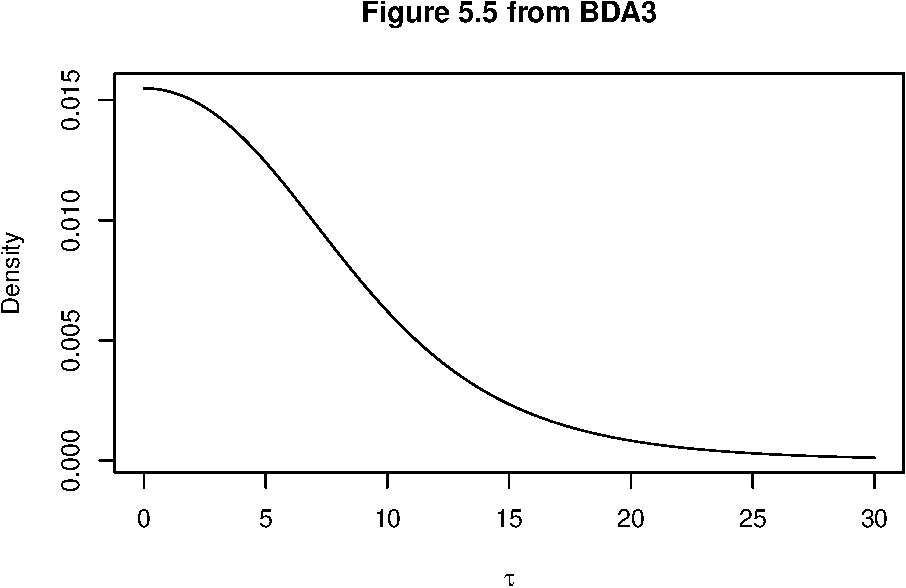
\includegraphics{Untitled_files/figure-latex/unnamed-chunk-8-1.pdf}

The sampling method in BDA3 suggest to apply the inverse method from the
posterior of \(\tau\). I don't do this for two reasons: (i) I'm not sure
the posterior has a closed for solution for its inverse, and (ii) given
that I already have the density, I can directly draw from that
distribution sampling using the \texttt{sample} command (which leads me
to think that this command applies the inverse method).

\begin{Shaded}
\begin{Highlighting}[]
\CommentTok{# Sampling}
\NormalTok{s.tau           <-}\StringTok{ }\KeywordTok{sample}\NormalTok{(tau.grid,samps,}\DataTypeTok{prob=}\NormalTok{pdf.tau, }\DataTypeTok{replace=}\OtherTok{TRUE}\NormalTok{)}
\NormalTok{s.mu            <-}\StringTok{ }\KeywordTok{sapply}\NormalTok{(s.tau,}\ControlFlowTok{function}\NormalTok{(x) }\KeywordTok{rnorm}\NormalTok{(}\DecValTok{1}\NormalTok{,}\KeywordTok{post.mu.hat}\NormalTok{(x),(}\KeywordTok{post.v.mu}\NormalTok{(x))}\OperatorTok{^}\FloatTok{0.5}\NormalTok{))}
\NormalTok{s.theta         <-}\StringTok{ }\OtherTok{NULL} 
\ControlFlowTok{for}\NormalTok{ (j }\ControlFlowTok{in} \DecValTok{1}\OperatorTok{:}\KeywordTok{length}\NormalTok{(school.id)) \{}
\NormalTok{  s.theta[[j]]         <-}\StringTok{ }\KeywordTok{sapply}\NormalTok{(}\DecValTok{1}\OperatorTok{:}\NormalTok{samps, }
                            \ControlFlowTok{function}\NormalTok{(x) }
                            \KeywordTok{rnorm}\NormalTok{(}\DecValTok{1}\NormalTok{,}
                                  \KeywordTok{post.theta.j}\NormalTok{(s.mu[x],s.tau[x],j),}
\NormalTok{                                  (}\KeywordTok{post.v.theta.j}\NormalTok{(s.tau[x],j))}\OperatorTok{^}\FloatTok{0.5}
\NormalTok{                                  ) )}
\NormalTok{  \}}
\end{Highlighting}
\end{Shaded}

\textbf{The following figures replicate the figures in pg 122 in BDA.
Before doing the plots we need to `average over \(\mu\)'}

\[
\begin{aligned}
E(\theta_{j}|\tau,y)   &= E_{\mu}\left[E(\theta_{j}|\tau,y,\mu)|\tau,y\right] \nonumber \\
                       &= E_{\mu}\left[\frac{ \frac{1}{\sigma_{j}^{2}}y_{j}  + \frac{1}{\tau^{2}}\mu }{\frac{1}{\sigma_{j}^{2}}  + \frac{1}{\tau^{2} } }|\tau,y\right] = \frac{ \frac{1}{\sigma_{j}^{2}}y_{j}  + \frac{1}{\tau^{2}}\hat{\mu} }{\frac{1}{\sigma_{j}^{2}}  + \frac{1}{\tau^{2} } }\\
\nonumber \\                       
Var(\theta_{j}|\tau,y) &= E_{\mu}\left[Var(\theta_{j}|\tau,y,\mu)|\tau,y\right] + Var_{\mu}\left[E(\theta_{j}|\tau,y,\mu)|\tau,y\right] \nonumber \\
                      &= \frac{1}{\frac{1}{\sigma_{j}^{2}}  + \frac{1}{\tau^{2} }} + V_{\mu}\left(\frac{\frac{1}{\tau^{2}}}{\frac{1}{\sigma_{j}^{2}}  + \frac{1}{\tau^{2} }}\right)
\end{aligned}
\]

Where \(V_{\mu}\) and \(\hat{\mu}\) correspond to the expressions
defined in Eq 5.20 of BDA3. Below is the code and plot of both
equations.

\begin{Shaded}
\begin{Highlighting}[]
\NormalTok{post.theta.j.no.mu     <-}\StringTok{ }\ControlFlowTok{function}\NormalTok{(tau,j) }\KeywordTok{post.theta.j}\NormalTok{( }\KeywordTok{post.mu.hat}\NormalTok{( tau ), tau, j )  }
\NormalTok{post.se.theta.j.no.mu  <-}\StringTok{ }\ControlFlowTok{function}\NormalTok{(tau,j) }\KeywordTok{sqrt}\NormalTok{( }
\NormalTok{  ( }\KeywordTok{post.v.theta.j}\NormalTok{( tau, j ) ) }\OperatorTok{*}\StringTok{ }\NormalTok{( }\DecValTok{1} \OperatorTok{+}\StringTok{ }\KeywordTok{post.v.mu}\NormalTok{( tau ) }\OperatorTok{*}\StringTok{ }\NormalTok{tau}\OperatorTok{^}\NormalTok{(}\OperatorTok{-}\DecValTok{2}\NormalTok{) ) )}

\KeywordTok{plot}\NormalTok{( tau.grid, }\KeywordTok{sapply}\NormalTok{(tau.grid, }\ControlFlowTok{function}\NormalTok{(x) }\KeywordTok{post.theta.j.no.mu}\NormalTok{(x,}\DecValTok{1}\NormalTok{) ), }
      \DataTypeTok{type=}\StringTok{"l"}\NormalTok{, }\DataTypeTok{ylim=}\KeywordTok{c}\NormalTok{(}\OperatorTok{-}\DecValTok{5}\NormalTok{,}\DecValTok{30}\NormalTok{), }
      \DataTypeTok{xlab=}\StringTok{""}\NormalTok{, }\DataTypeTok{ylab=}\StringTok{""}\NormalTok{)}
\KeywordTok{title}\NormalTok{(}\DataTypeTok{main=}\StringTok{"Figure 5.6 from BDA3"}\NormalTok{, }
      \DataTypeTok{xlab=}\KeywordTok{expression}\NormalTok{(tau), }
      \DataTypeTok{ylab=}\StringTok{"Estimated treatment effect"}\NormalTok{)}

\ControlFlowTok{for}\NormalTok{ (j }\ControlFlowTok{in} \DecValTok{2}\OperatorTok{:}\DecValTok{8}\NormalTok{) \{ }
  \KeywordTok{lines}\NormalTok{( tau.grid, }
         \KeywordTok{sapply}\NormalTok{( tau.grid, }\ControlFlowTok{function}\NormalTok{(x) }\KeywordTok{post.theta.j.no.mu}\NormalTok{(x,j) ) )}
\NormalTok{\}}
\end{Highlighting}
\end{Shaded}

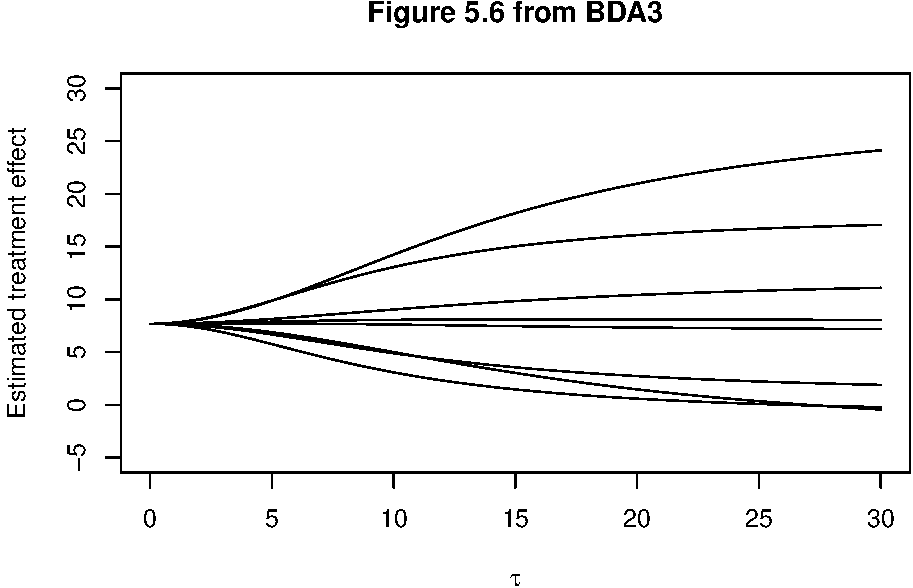
\includegraphics{Untitled_files/figure-latex/unnamed-chunk-10-1.pdf}

\begin{Shaded}
\begin{Highlighting}[]
\KeywordTok{plot}\NormalTok{( tau.grid, }\KeywordTok{sapply}\NormalTok{(tau.grid, }\ControlFlowTok{function}\NormalTok{(x) }\KeywordTok{post.se.theta.j.no.mu}\NormalTok{(x,}\DecValTok{1}\NormalTok{) ), }
      \DataTypeTok{type=}\StringTok{"l"}\NormalTok{, }\DataTypeTok{ylim=}\KeywordTok{c}\NormalTok{(}\DecValTok{0}\NormalTok{,}\DecValTok{20}\NormalTok{),}
      \DataTypeTok{xlab=}\StringTok{""}\NormalTok{, }\DataTypeTok{ylab=}\StringTok{""}\NormalTok{)}
\KeywordTok{title}\NormalTok{(}\DataTypeTok{main=}\StringTok{"Figure 5.7 from BDA3"}\NormalTok{, }
      \DataTypeTok{xlab=}\KeywordTok{expression}\NormalTok{(tau), }
      \DataTypeTok{ylab=}\StringTok{"Posterior Standard Deviation"}\NormalTok{)}

\ControlFlowTok{for}\NormalTok{ (j }\ControlFlowTok{in} \DecValTok{2}\OperatorTok{:}\DecValTok{8}\NormalTok{) \{ }
  \KeywordTok{lines}\NormalTok{( tau.grid, }
         \KeywordTok{sapply}\NormalTok{( tau.grid, }\ControlFlowTok{function}\NormalTok{(x) }\KeywordTok{post.se.theta.j.no.mu}\NormalTok{(x,j) ) )}
\NormalTok{\}}
\end{Highlighting}
\end{Shaded}

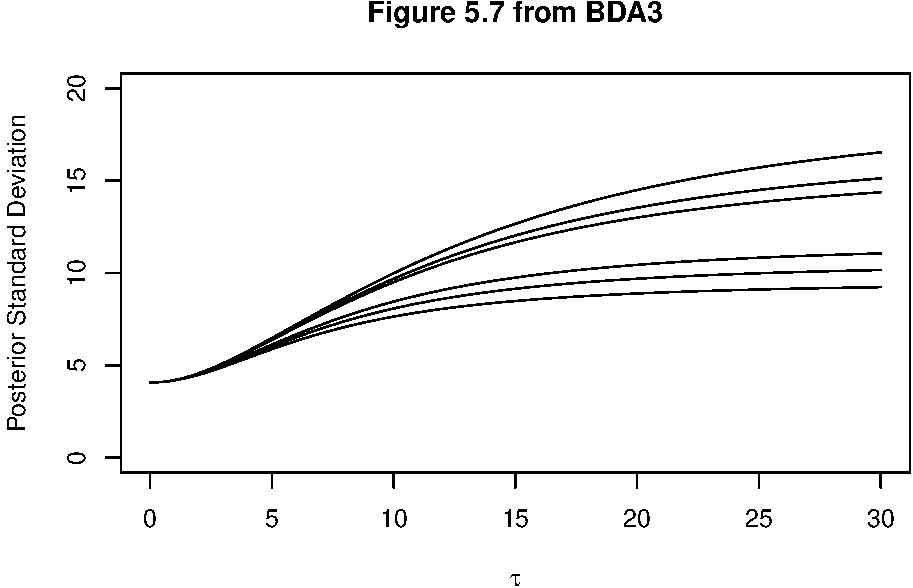
\includegraphics{Untitled_files/figure-latex/unnamed-chunk-10-2.pdf}

\begin{Shaded}
\begin{Highlighting}[]
\NormalTok{s.theta         <-}\StringTok{ }\KeywordTok{matrix}\NormalTok{(}\KeywordTok{unlist}\NormalTok{(s.theta), }\DataTypeTok{ncol =} \DecValTok{8}\NormalTok{, }\DataTypeTok{byrow =} \OtherTok{FALSE}\NormalTok{)}
\NormalTok{s.theta.sort    <-}\StringTok{ }\KeywordTok{apply}\NormalTok{(s.theta, }\DecValTok{2}\NormalTok{, sort)}
\NormalTok{p               <-}\StringTok{ }\KeywordTok{t}\NormalTok{( }\KeywordTok{apply}\NormalTok{( s.theta.sort, }\DecValTok{2}\NormalTok{, }\ControlFlowTok{function}\NormalTok{(x) }
            \KeywordTok{quantile}\NormalTok{( x, }\KeywordTok{c}\NormalTok{( .}\DecValTok{025}\NormalTok{, .}\DecValTok{25}\NormalTok{, .}\DecValTok{5}\NormalTok{, .}\DecValTok{75}\NormalTok{, .}\DecValTok{975}\NormalTok{), }\DataTypeTok{type=}\DecValTok{1}\NormalTok{ ) ) )}
\NormalTok{p               <-}\StringTok{ }\KeywordTok{round}\NormalTok{(p,}\DecValTok{3}\NormalTok{)}
\CommentTok{#Bug in line below}
\CommentTok{#knitr::kable(p, caption="Misclassification and Reliability for Different Thresholds")}
\end{Highlighting}
\end{Shaded}

\textbf{Table 5.3 from BDA3: }\\
Now we can use the simulated \(\theta_s\) to described the estimated
effects in each school.

\begin{longtable}[]{@{}rccccc@{}}
\toprule
School & & & & &\tabularnewline
\midrule
\endhead
& 2.5\% & 25\% & median & 75\% & 97.5\%\tabularnewline
A & -1.287 & 6.127 & 9.702 & 14.719 & 32.959\tabularnewline
B & -5.205 & 3.904 & 7.958 & 11.727 & 22.622\tabularnewline
C & -11.529 & 1.932 & 7.345 & 11.119 & 21.305\tabularnewline
D & -4.456 & 3.535 & 7.369 & 11.092 & 19.771\tabularnewline
E & -11.326 & 0.956 & 6.303 & 9.364 & 18.245\tabularnewline
F & -5.954 & 2.578 & 6.999 & 10.396 & 17.554\tabularnewline
G & -0.544 & 7.096 & 10.007 & 14.477 & 26.717\tabularnewline
H & -6.289 & 3.54 & 7.725 & 11.798 & 22.223\tabularnewline
\bottomrule
\end{longtable}

Here we reproduce figure 5.8

\begin{Shaded}
\begin{Highlighting}[]
\KeywordTok{par}\NormalTok{(}\DataTypeTok{mfrow=}\KeywordTok{c}\NormalTok{(}\DecValTok{1}\NormalTok{,}\DecValTok{2}\NormalTok{))  }
\NormalTok{domain           <-}\StringTok{ }\KeywordTok{c}\NormalTok{(}\OperatorTok{-}\DecValTok{20}\NormalTok{,}\DecValTok{60}\NormalTok{)}
\KeywordTok{hist}\NormalTok{(s.theta[,}\DecValTok{1}\NormalTok{], }\DataTypeTok{breaks=}\DecValTok{10}\NormalTok{, }\DataTypeTok{xlab=}\StringTok{"Effect in School A"}\NormalTok{, }\DataTypeTok{main=}\StringTok{""}\NormalTok{, }\DataTypeTok{xlim=}\NormalTok{domain)}
\KeywordTok{hist}\NormalTok{(}\KeywordTok{apply}\NormalTok{(s.theta,}\DecValTok{1}\NormalTok{,max), }\DataTypeTok{breaks=}\DecValTok{10}\NormalTok{, }\DataTypeTok{xlab=}\StringTok{"Largest Effect"}\NormalTok{, }\DataTypeTok{main=}\StringTok{""}\NormalTok{, }\DataTypeTok{xlim=}\NormalTok{domain)}
\KeywordTok{title}\NormalTok{(}\DataTypeTok{main=}\StringTok{"Figure 5.8 from BDA3"}\NormalTok{)}
\end{Highlighting}
\end{Shaded}

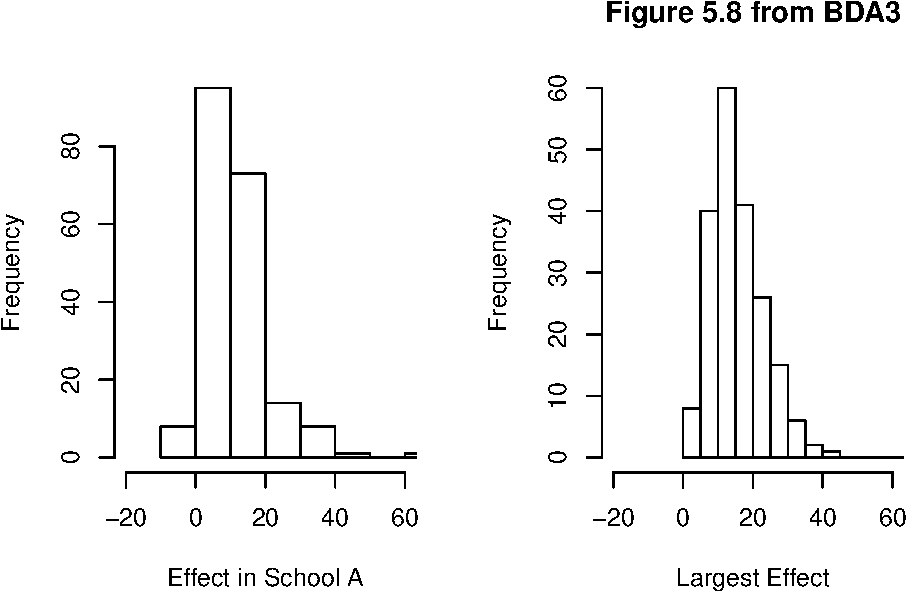
\includegraphics{Untitled_files/figure-latex/unnamed-chunk-12-1.pdf}

This last figure (``largest effect'') is a good example of one the main
advantage of a fully Bayesian hierarchical model: once we have simulated
the posterior, we can test all kinds of complicated hypothesis.

\subsubsection{5.3a}\label{a-3}

\begin{itemize}
\item
  \begin{enumerate}
  \def\labelenumi{(\roman{enumi})}
  \tightlist
  \item
    For each school \(j\), the probability that its coaching program is
    the best of eight:\\
    (\textbf{Important:} do not sort each posterior).
  \end{enumerate}
\end{itemize}

\begin{Shaded}
\begin{Highlighting}[]
\NormalTok{aux1            <-}\StringTok{ }\KeywordTok{apply}\NormalTok{(s.theta,}\DecValTok{1}\NormalTok{,max)}
\NormalTok{best            <-}\StringTok{ }\KeywordTok{apply}\NormalTok{(}\DecValTok{1}\OperatorTok{*}\NormalTok{(s.theta}\OperatorTok{==}\NormalTok{aux1), }\DecValTok{2}\NormalTok{,mean)}
\end{Highlighting}
\end{Shaded}

\textbf{Table 2: Probability that each coaching program is the best
among the eight schools}

\begin{longtable}[]{@{}rc@{}}
\toprule
School & Probability of having the best coaching program\tabularnewline
\midrule
\endhead
A & 0.275\tabularnewline
B & 0.11\tabularnewline
C & 0.055\tabularnewline
D & 0.09\tabularnewline
E & 0.06\tabularnewline
F & 0.075\tabularnewline
G & 0.23\tabularnewline
H & 0.105\tabularnewline
\bottomrule
\end{longtable}

\begin{itemize}
\item
  \begin{enumerate}
  \def\labelenumi{(\roman{enumi})}
  \setcounter{enumi}{1}
  \tightlist
  \item
    For each school \(j\), the probability that its coaching program is
    better than other school \(k\):
  \end{enumerate}
\end{itemize}

\begin{Shaded}
\begin{Highlighting}[]
\NormalTok{p               <-}\StringTok{ }\KeywordTok{sapply}\NormalTok{( }\DecValTok{1}\OperatorTok{:}\DecValTok{8}\NormalTok{,}
                          \ControlFlowTok{function}\NormalTok{(y) }\KeywordTok{sapply}\NormalTok{( }\DecValTok{1}\OperatorTok{:}\DecValTok{8}\NormalTok{,}
                                             \ControlFlowTok{function}\NormalTok{(x) }
                                               \KeywordTok{mean}\NormalTok{( }\DecValTok{1} \OperatorTok{*}\StringTok{ }\NormalTok{( s.theta[,x] }\OperatorTok{>}\StringTok{ }\NormalTok{s.theta[,y] ) ) }
\NormalTok{                                             ) }
\NormalTok{                          )}
\end{Highlighting}
\end{Shaded}

\pagebreak

\textbf{Table 3: Probability that school \(j\) (row) has a better
program that school \(k\) (column)}

\begin{longtable}[]{@{}rcccccccc@{}}
\toprule
School \(j\)/School \(k\) & & & & & & & &\tabularnewline
\midrule
\endhead
& A & B & C & D & E & F & G & H\tabularnewline
A & 0 & 0.64 & 0.7 & 0.655 & 0.725 & 0.69 & 0.49 & 0.625\tabularnewline
B & 0.36 & 0 & 0.565 & 0.54 & 0.66 & 0.58 & 0.365 & 0.475\tabularnewline
C & 0.3 & 0.435 & 0 & 0.465 & 0.555 & 0.48 & 0.3 & 0.42\tabularnewline
D & 0.345 & 0.46 & 0.535 & 0 & 0.62 & 0.545 & 0.355 &
0.49\tabularnewline
E & 0.275 & 0.34 & 0.445 & 0.38 & 0 & 0.425 & 0.275 &
0.385\tabularnewline
F & 0.31 & 0.42 & 0.52 & 0.455 & 0.575 & 0 & 0.295 & 0.43\tabularnewline
G & 0.51 & 0.635 & 0.7 & 0.645 & 0.725 & 0.705 & 0 &
0.625\tabularnewline
H & 0.375 & 0.525 & 0.58 & 0.51 & 0.615 & 0.57 & 0.375 &
0\tabularnewline
\bottomrule
\end{longtable}

\subsubsection{5.3b}\label{b-2}

\begin{itemize}
\item
  \begin{enumerate}
  \def\labelenumi{(\roman{enumi})}
  \tightlist
  \item
    Now with \(\tau = \infty\) compute for each school \(j\), the
    probability that it has the best coaching program:\\
    With \(\tau = \infty\) each school posterior effect is independent
    \(\theta_{j} \sim N(y_{y}, \sigma_{j}^{2})\). The probability of a
    school having the best coaching program is:\\
    \textbf{Wrong way to do it:}\\
    \[
    \begin{aligned}  
    p(\theta_{j}>max_{i\neq j}\{\theta_{i}\}) &= \prod_{i\neq j} p(\theta_{j}>\theta_{i}) \\
                                      &= \prod_{i\neq j} \Phi(\frac{\theta_{j} - \theta_{i}}{\sigma_{i}})  
    \end{aligned}
    \]
  \end{enumerate}
\end{itemize}

\textbf{Right way to do it:}\\
\[
\begin{aligned}  
p(\theta_{j}>max_{i\neq j}\{\theta_{i}\}) &= \int \prod_{i\neq j} p(\theta_{j}>\theta_{i}) \phi(\theta_{j}|y_{j},\sigma_{j})d\theta_{j} \\
                                          &= \int \prod_{i\neq j} \Phi\left(\frac{\theta_{j} - \theta_{i}}{\sigma_{i}}\right) \phi(\theta_{j}|y_{j},\sigma_{j})d\theta_{j}                               
\end{aligned}
\]

This integral has to be solved numerically:

\begin{Shaded}
\begin{Highlighting}[]
\KeywordTok{set.seed}\NormalTok{(}\DecValTok{142857}\NormalTok{)}
\NormalTok{best            <-}\StringTok{  }\KeywordTok{sapply}\NormalTok{(}\DecValTok{1}\OperatorTok{:}\DecValTok{8}\NormalTok{,}
                      \ControlFlowTok{function}\NormalTok{(y) }\KeywordTok{mean}\NormalTok{( }\KeywordTok{sapply}\NormalTok{( }\DecValTok{1}\OperatorTok{:}\DecValTok{1000}\NormalTok{ ,}
                        \ControlFlowTok{function}\NormalTok{(x) }
                          \KeywordTok{prod}\NormalTok{( }\KeywordTok{pnorm}\NormalTok{( ( }
                            \KeywordTok{rnorm}\NormalTok{( }\DecValTok{1}\NormalTok{ , effect[y] , se.effect[y] ) }\OperatorTok{-}\StringTok{ }\NormalTok{effect[}\OperatorTok{-}\NormalTok{y] ) }\OperatorTok{/}\StringTok{ }
\StringTok{                              }\NormalTok{se.effect[}\OperatorTok{-}\NormalTok{y] ) ) )}
\NormalTok{                           )}
\NormalTok{                           )}
\CommentTok{# Ad-hoc normalization:}
\NormalTok{best            <-}\StringTok{ }\NormalTok{best}\OperatorTok{/}\KeywordTok{sum}\NormalTok{(best)  }
\end{Highlighting}
\end{Shaded}

\textbf{Table 4: Probability that each coaching program is the best
among the eight schools (with \(\tau = \infty\))}

\begin{longtable}[]{@{}rc@{}}
\toprule
School & Probability of having the best coaching program\tabularnewline
\midrule
\endhead
A & 0.559927\tabularnewline
B & 0.0329844\tabularnewline
C & 0.0265477\tabularnewline
D & 0.0364362\tabularnewline
E & 0.0034413\tabularnewline
F & 0.0136409\tabularnewline
G & 0.1614563\tabularnewline
H & 0.1655662\tabularnewline
\bottomrule
\end{longtable}

\begin{itemize}
\item
  \begin{enumerate}
  \def\labelenumi{(\roman{enumi})}
  \setcounter{enumi}{1}
  \tightlist
  \item
    Now with \(\tau = \infty\) compute for each school \(j\), the
    probability that its coaching program is the better than other
    school \(k\):\\
    \[
    \begin{aligned}  
    p(\theta_{i}>\theta_{j}) &= p\left(-\frac{y_{j} - y_{i}}{\sqrt{\sigma_{i}^{2} + \sigma_{j}^{2}}} > \frac{(\theta_{j}-\theta_{i})- (y_{j} - y_{i})}{\sqrt{\sigma_{i}^{2} + \sigma_{j}^{2}}} \right) \\
                     &= \Phi\left( \frac{y_{i} - y_{j}}{\sqrt{\sigma_{i}^{2} + \sigma_{j}^{2}}}\right)
    \end{aligned}
    \]
  \end{enumerate}
\end{itemize}

The following table presents the different values for the expression
above:

\begin{Shaded}
\begin{Highlighting}[]
\NormalTok{p               <-}\StringTok{ }\KeywordTok{sapply}\NormalTok{(}\DecValTok{1}\OperatorTok{:}\DecValTok{8}\NormalTok{,}\ControlFlowTok{function}\NormalTok{(x) }
                   \KeywordTok{sapply}\NormalTok{(}\DecValTok{1}\OperatorTok{:}\DecValTok{8}\NormalTok{,}\ControlFlowTok{function}\NormalTok{(y) }
                  \KeywordTok{pnorm}\NormalTok{( }\DataTypeTok{q =} \DecValTok{0}\NormalTok{, }\DataTypeTok{mean =}\NormalTok{ (effect[x] }\OperatorTok{-}\StringTok{ }\NormalTok{effect[y]) }\OperatorTok{/}\StringTok{ }\KeywordTok{sqrt}\NormalTok{(se.effect[x]}\OperatorTok{^}\DecValTok{2} \OperatorTok{+}\StringTok{ }\NormalTok{se.effect[y]}\OperatorTok{^}\DecValTok{2}\NormalTok{) , }
                  \DataTypeTok{sd =} \DecValTok{1}\NormalTok{ )}
\NormalTok{                  ) )  }
\CommentTok{# Force all elementens in the diagonal to zero. }
\NormalTok{p               <-}\StringTok{ }\NormalTok{p }\OperatorTok{-}\StringTok{ }\NormalTok{.}\DecValTok{5} \OperatorTok{*}\StringTok{ }\KeywordTok{diag}\NormalTok{(}\DecValTok{8}\NormalTok{)}
\end{Highlighting}
\end{Shaded}

\textbf{Table 5: Probability that \(j\) (row) has a better program that
school \(k\) (column). With \(\tau = \infty\)}

\begin{longtable}[]{@{}rcccccccc@{}}
\toprule
School \(j\)/School \(k\) & & & & & & & &\tabularnewline
\midrule
\endhead
& A & B & C & D & E & F & G & H\tabularnewline
A & 0 & 0.8663713 & 0.9212424 & 0.8705441 & 0.9513231 & 0.9266837 &
0.7104501 & 0.7526534\tabularnewline
B & 0.1336287 & 0 & 0.720053 & 0.5268155 & 0.748241 & 0.6811336 &
0.2397501 & 0.4229873\tabularnewline
C & 0.0787576 & 0.279947 & 0 & 0.3032674 & 0.4566223 & 0.4183914 &
0.1328547 & 0.2666945\tabularnewline
D & 0.1294559 & 0.4731845 & 0.6967326 & 0 & 0.713241 & 0.6501386 &
0.2296682 & 0.4063196\tabularnewline
E & 0.0486769 & 0.251759 & 0.5433777 & 0.286759 & 0 & 0.4440458 &
0.0789369 & 0.2591477\tabularnewline
F & 0.0733163 & 0.3188664 & 0.5816086 & 0.3498614 & 0.5559542 & 0 &
0.1264065 & 0.3010267\tabularnewline
G & 0.2895499 & 0.7602499 & 0.8671453 & 0.7703318 & 0.9210631 &
0.8735935 & 0 & 0.6146218\tabularnewline
H & 0.2473466 & 0.5770127 & 0.7333055 & 0.5936804 & 0.7408523 &
0.6989733 & 0.3853782 & 0\tabularnewline
\bottomrule
\end{longtable}

\subsubsection{5.3c}\label{c-2}

The estimated differences between the closed form solutions (5.3b) and
the bayesian analysis (5.3a) is that the latter presents less extreme
probability estimates (shrinkage)

\subsubsection{5.3d}\label{d-1}

If \(\tau = 0\), then all effects are the same so the probabilities can
be 0 or 1 for all schools (all are the largest effect and the smallest
at the same time)

\subsection{5.13 - Bicycles}\label{bicycles}

\begin{Shaded}
\begin{Highlighting}[]
\CommentTok{#Load data}
\NormalTok{y                <-}\StringTok{ }\KeywordTok{c}\NormalTok{(}\DecValTok{16}\NormalTok{, }\DecValTok{9}\NormalTok{  , }\DecValTok{10}\NormalTok{ , }\DecValTok{13}\NormalTok{ , }\DecValTok{19}\NormalTok{ , }\DecValTok{20}\NormalTok{ , }\DecValTok{18}\NormalTok{ , }\DecValTok{17}\NormalTok{ , }\DecValTok{35}\NormalTok{ , }\DecValTok{55}\NormalTok{ )}
\NormalTok{n                <-}\StringTok{ }\KeywordTok{c}\NormalTok{(}\DecValTok{74}\NormalTok{, }\DecValTok{99}\NormalTok{ , }\DecValTok{58}\NormalTok{ , }\DecValTok{70}\NormalTok{ , }\DecValTok{122}\NormalTok{, }\DecValTok{77}\NormalTok{ , }\DecValTok{104}\NormalTok{, }\DecValTok{129}\NormalTok{, }\DecValTok{308}\NormalTok{, }\DecValTok{119}\NormalTok{)}
\end{Highlighting}
\end{Shaded}

\subsubsection{5.13a}\label{a-4}

\(y_{i}\sim Bin(\theta_{i},n_{i})\) where \(n_{i}\) represents the
\emph{total} number of vehicles (bicycles + other vehicles).
\(\theta_{i}\sim Beta(\alpha,\beta)\) the prior distribution of biking
rates for each street. We set a non-informative hyper-prior
\(p(\alpha,\beta) \propto (\alpha + \beta)^{-5/2}\). This implies that
the \textbf{joint posterior} distribution has the following (same as in
equation 5.6 in BDA3):

\[
\begin{aligned}
p(\theta,\alpha,\beta|y) &\propto p(\alpha, \beta)p(\theta|\alpha, \beta)p(y|\theta,\alpha, \beta) \nonumber \\ 
p(\theta,\alpha,\beta|y) &\propto p(\alpha, \beta)\prod^{J}_{j=1} \frac{\Gamma(\alpha + \beta)}{\Gamma(\alpha)\Gamma(\beta)} \theta_{j}^{\alpha - 1} (1 - \theta_{j})^{\beta - 1}\prod^{J}_{j=1} \theta_{j}^{y_{j}} (1 - \theta_{j})^{n_{j}-y_{j}}\label{bic.joint.post1}
\end{aligned}
\]

\subsubsection{5.13b}\label{b-3}

Compute the marginal posterior of \(\theta\), conditional on
\(\alpha, \beta\). For the beta-binomial case we have that given the
hyper-parameters, each \(\theta_{j}\) has a posterior distribution
\(Beta(\alpha + y_{j}, \beta +n_{j} - y_{j})\). Assuming
exchangeability: \[
\begin{aligned}
p(\theta|\alpha,\beta,y) &= \prod^{J}_{j=1} \frac{\Gamma(\alpha + \beta +n_{j})}{\Gamma(\alpha+y_{j})\Gamma(\beta+n_{j}-y_{j})} \theta_{j}^{\alpha+y_{j} - 1} (1 - \theta_{j})^{\beta+n_{j}-y_{j} - 1}\label{bic.cond.post.theta1}
\end{aligned}
\]

Now we compute the posterior marginal of \((\alpha,\beta)\). Given that
we do have a closed form solution in step 2, we compute the ratio of
(\textbackslash{}ref\{bic.joint.post1\}) and
(\textbackslash{}ref\{bic.cond.post.theta1\}).

\[
\begin{aligned}
p(\alpha,\beta|y) &\propto \prod^{J}_{j=1} \frac{\Gamma(\alpha + \beta)}{\Gamma(\alpha)\Gamma(\beta)} \frac{\Gamma(\alpha+y_{j})\Gamma(\beta+n_{j}-y_{j})}{\Gamma(\alpha + \beta +n_{j})} \label{rat.marg.post.phi1}
\end{aligned}
\]

Centering our grid around the methods of moments estimates for
\((\alpha_{0}, \beta_{0})\):

\[
\begin{aligned}
\hat{\mu}     &= 0.1961412 = \frac{\hat{\alpha_{0}}}{\hat{\alpha_{0}}+\hat{\beta_{0}}}\\
\hat{\sigma^2} &= 0.0111207   = \frac{\hat{\alpha_{0}}\hat{\beta_{0}}}{(\hat{\alpha_{0}}+\hat{\beta_{0}})^{2}(\hat{\alpha_{0}}+\hat{\beta_{0}}+1)}
\end{aligned}
\]

Solving form \((\hat{\alpha_{0}},\hat{\beta_{0}})\):

\begin{Shaded}
\begin{Highlighting}[]
\CommentTok{#Here 'x' represents alpha and beta}
\NormalTok{dslnex          <-}\StringTok{ }\ControlFlowTok{function}\NormalTok{(x) \{}
\NormalTok{    z           <-}\StringTok{ }\KeywordTok{numeric}\NormalTok{(}\DecValTok{2}\NormalTok{)}
\NormalTok{    z[}\DecValTok{1}\NormalTok{]        <-}\StringTok{ }\NormalTok{x[}\DecValTok{1}\NormalTok{]}\OperatorTok{/}\NormalTok{(x[}\DecValTok{1}\NormalTok{]}\OperatorTok{+}\NormalTok{x[}\DecValTok{2}\NormalTok{]) }\OperatorTok{-}\StringTok{ }\KeywordTok{mean}\NormalTok{(y}\OperatorTok{/}\NormalTok{n)}
\NormalTok{    z[}\DecValTok{2}\NormalTok{]        <-}\StringTok{ }\NormalTok{x[}\DecValTok{1}\NormalTok{]}\OperatorTok{*}\NormalTok{x[}\DecValTok{2}\NormalTok{]}\OperatorTok{/}\NormalTok{(((x[}\DecValTok{1}\NormalTok{]}\OperatorTok{+}\NormalTok{x[}\DecValTok{2}\NormalTok{])}\OperatorTok{^}\DecValTok{2}\NormalTok{)}\OperatorTok{*}\NormalTok{(x[}\DecValTok{1}\NormalTok{]}\OperatorTok{+}\NormalTok{x[}\DecValTok{2}\NormalTok{]}\OperatorTok{+}\DecValTok{1}\NormalTok{)) }\OperatorTok{-}\StringTok{ }\KeywordTok{sd}\NormalTok{(y}\OperatorTok{/}\NormalTok{n)}\OperatorTok{^}\DecValTok{2}
\NormalTok{    z}
\NormalTok{\}}

\NormalTok{sol1            <-}\StringTok{ }\KeywordTok{nleqslv}\NormalTok{(}\KeywordTok{c}\NormalTok{(}\DecValTok{1}\NormalTok{,}\DecValTok{1}\NormalTok{), dslnex) }
\NormalTok{res1            <-}\StringTok{ }\KeywordTok{paste}\NormalTok{(}\StringTok{"("}\NormalTok{,}\KeywordTok{round}\NormalTok{(sol1}\OperatorTok{$}\NormalTok{x[}\DecValTok{1}\NormalTok{],}\DecValTok{1}\NormalTok{), }\StringTok{","}\NormalTok{, }\KeywordTok{round}\NormalTok{(sol1}\OperatorTok{$}\NormalTok{x[}\DecValTok{2}\NormalTok{],}\DecValTok{1}\NormalTok{), }\StringTok{")"}\NormalTok{,}\DataTypeTok{sep=}\StringTok{""}\NormalTok{)}
\end{Highlighting}
\end{Shaded}

We get: \((\hat{\alpha_{0}},\hat{\beta_{0}}) = (2.6,10.6)\).

We center the grid (approximately) around that initial estimate and
expand the grid to cover up to a factor of 4 of each parameter. The
result is plotted in the following figure:

\begin{Shaded}
\begin{Highlighting}[]
\NormalTok{bic.marg.post.phi <-}\StringTok{   }\ControlFlowTok{function}\NormalTok{(alpha, beta) \{}
\NormalTok{  post          <-}\StringTok{  }\DecValTok{1}
  \CommentTok{#notice the censoring in n (the gamma(.) function in R cannot handle large values)}
  \ControlFlowTok{for}\NormalTok{ (i }\ControlFlowTok{in} \DecValTok{1}\OperatorTok{:}\KeywordTok{length}\NormalTok{(y)) \{}
    \ControlFlowTok{if}\NormalTok{ (n[i] }\OperatorTok{>}\StringTok{ }\DecValTok{100}\NormalTok{) n[i] =}\StringTok{ }\DecValTok{100}
\NormalTok{    post  =}\StringTok{ }\NormalTok{post }\OperatorTok{*}\StringTok{ }\NormalTok{( }
\NormalTok{      ( ( }\KeywordTok{gamma}\NormalTok{(alpha }\OperatorTok{+}\StringTok{ }\NormalTok{beta) ) }\OperatorTok{/}\StringTok{ }
\StringTok{        }\NormalTok{( }\KeywordTok{gamma}\NormalTok{(alpha) }\OperatorTok{*}\StringTok{ }\KeywordTok{gamma}\NormalTok{(beta) ) ) }\OperatorTok{*}\StringTok{ }
\StringTok{      }\NormalTok{( ( }\KeywordTok{gamma}\NormalTok{(alpha }\OperatorTok{+}\StringTok{ }\NormalTok{y[i] ) }\OperatorTok{*}\StringTok{ }\KeywordTok{gamma}\NormalTok{(beta }\OperatorTok{+}\StringTok{ }\NormalTok{n[i] }\OperatorTok{-}\StringTok{ }\NormalTok{y[i]) ) }\OperatorTok{/}\StringTok{ }
\StringTok{        }\NormalTok{( }\KeywordTok{gamma}\NormalTok{(alpha }\OperatorTok{+}\StringTok{ }\NormalTok{beta }\OperatorTok{+}\StringTok{ }\NormalTok{n[i]) ) ) }
\NormalTok{      )}
\NormalTok{  \}}
  \CommentTok{# The hyper prior is defined below}
  \KeywordTok{bic.hyper.prior}\NormalTok{(alpha,beta) }\OperatorTok{*}\StringTok{ }\NormalTok{post}
\NormalTok{\}}

\NormalTok{bic.hyper.prior <-}\StringTok{  }\ControlFlowTok{function}\NormalTok{(alpha,beta) }
\NormalTok{\{}
\NormalTok{    alpha}\OperatorTok{*}\NormalTok{beta}\OperatorTok{*}\NormalTok{(alpha }\OperatorTok{+}\StringTok{ }\NormalTok{beta)}\OperatorTok{^}\NormalTok{(}\OperatorTok{-}\DecValTok{5}\OperatorTok{/}\DecValTok{2}\NormalTok{)}
\NormalTok{\}}

\NormalTok{v1              <-}\StringTok{  }\KeywordTok{seq}\NormalTok{(}\KeywordTok{log}\NormalTok{(sol1}\OperatorTok{$}\NormalTok{x[}\DecValTok{1}\NormalTok{]}\OperatorTok{/}\NormalTok{sol1}\OperatorTok{$}\NormalTok{x[}\DecValTok{2}\NormalTok{])}\OperatorTok{*}\FloatTok{1.5}\NormalTok{,}
                        \KeywordTok{log}\NormalTok{(sol1}\OperatorTok{$}\NormalTok{x[}\DecValTok{1}\NormalTok{]}\OperatorTok{/}\NormalTok{sol1}\OperatorTok{$}\NormalTok{x[}\DecValTok{2}\NormalTok{])}\OperatorTok{/}\FloatTok{1.5}\NormalTok{,}\DataTypeTok{length.out =}\DecValTok{151}\NormalTok{)}
\NormalTok{v2              <-}\StringTok{  }\KeywordTok{seq}\NormalTok{(}\KeywordTok{log}\NormalTok{(sol1}\OperatorTok{$}\NormalTok{x[}\DecValTok{1}\NormalTok{]}\OperatorTok{+}\NormalTok{sol1}\OperatorTok{$}\NormalTok{x[}\DecValTok{2}\NormalTok{])}\OperatorTok{/}\FloatTok{1.5}\NormalTok{,}
                        \KeywordTok{log}\NormalTok{(sol1}\OperatorTok{$}\NormalTok{x[}\DecValTok{1}\NormalTok{]}\OperatorTok{+}\NormalTok{sol1}\OperatorTok{$}\NormalTok{x[}\DecValTok{2}\NormalTok{])}\OperatorTok{*}\FloatTok{1.5}\NormalTok{,}\DataTypeTok{length.out =}\DecValTok{151}\NormalTok{)}
\NormalTok{beta            <-}\StringTok{  }\KeywordTok{exp}\NormalTok{(v2)}\OperatorTok{/}\NormalTok{(}\KeywordTok{exp}\NormalTok{(v1)}\OperatorTok{+}\DecValTok{1}\NormalTok{)}
\NormalTok{alpha           <-}\StringTok{  }\KeywordTok{exp}\NormalTok{(v2}\OperatorTok{+}\NormalTok{v1)}\OperatorTok{/}\NormalTok{(}\KeywordTok{exp}\NormalTok{(v1)}\OperatorTok{+}\DecValTok{1}\NormalTok{)}

\NormalTok{post.dens       <-}\StringTok{  }\KeywordTok{outer}\NormalTok{(alpha,beta,}\ControlFlowTok{function}\NormalTok{(x1,x2) }\KeywordTok{log}\NormalTok{(}\KeywordTok{bic.marg.post.phi}\NormalTok{(x1, x2)) )}
\NormalTok{post.dens       <-}\StringTok{  }\KeywordTok{exp}\NormalTok{(post.dens }\OperatorTok{-}\StringTok{ }\KeywordTok{max}\NormalTok{(post.dens))}
\NormalTok{post.dens       <-}\StringTok{  }\NormalTok{post.dens}\OperatorTok{/}\KeywordTok{sum}\NormalTok{(post.dens)}

\NormalTok{contours        <-}\StringTok{  }\KeywordTok{seq}\NormalTok{(}\KeywordTok{min}\NormalTok{(post.dens), }\KeywordTok{max}\NormalTok{(post.dens) , }\DataTypeTok{length=}\DecValTok{10}\NormalTok{)}
\KeywordTok{contour}\NormalTok{(v1, v2, post.dens,}
        \DataTypeTok{levels=}\NormalTok{contours, }
        \DataTypeTok{xlab=}\KeywordTok{expression}\NormalTok{( }\KeywordTok{log}\NormalTok{(alpha}\OperatorTok{/}\NormalTok{beta) ), }
        \DataTypeTok{ylab=}\KeywordTok{expression}\NormalTok{( }\KeywordTok{log}\NormalTok{(alpha}\OperatorTok{+}\NormalTok{beta) ), }
        \DataTypeTok{xlim=}\KeywordTok{c}\NormalTok{( }\KeywordTok{min}\NormalTok{( v1 ), }\KeywordTok{max}\NormalTok{( v1 ) ) , }
        \DataTypeTok{ylim=}\KeywordTok{c}\NormalTok{( }\KeywordTok{min}\NormalTok{( v2 ), }\KeywordTok{max}\NormalTok{( v2 ) ), }
        \DataTypeTok{drawlabels=}\OtherTok{FALSE}\NormalTok{, }
        \DataTypeTok{main=}\StringTok{"Contour plot of joint posterior"}\NormalTok{)}
\end{Highlighting}
\end{Shaded}

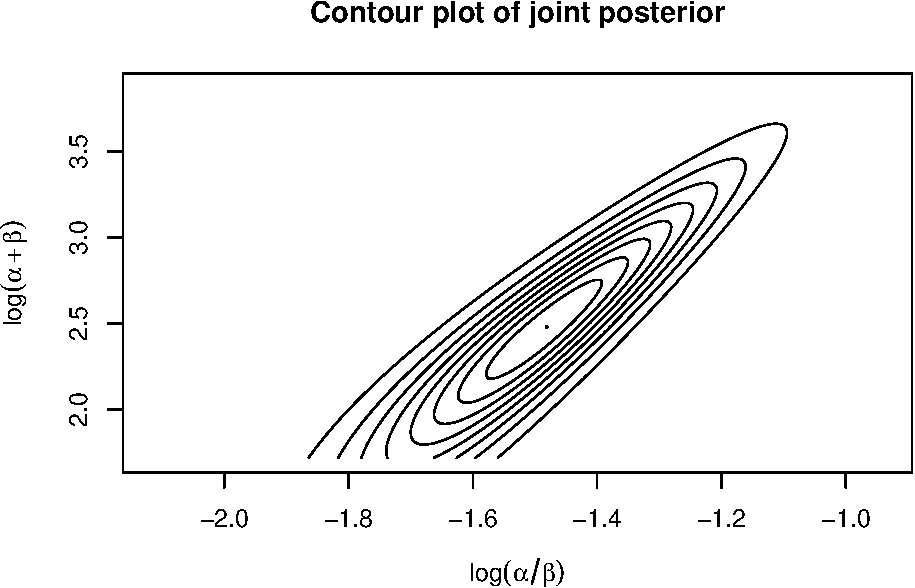
\includegraphics{Untitled_files/figure-latex/unnamed-chunk-18-1.pdf}

Adjust the grid and repeat:

\begin{Shaded}
\begin{Highlighting}[]
\NormalTok{v1              <-}\StringTok{  }\KeywordTok{seq}\NormalTok{(}\KeywordTok{log}\NormalTok{(sol1}\OperatorTok{$}\NormalTok{x[}\DecValTok{1}\NormalTok{]}\OperatorTok{/}\NormalTok{sol1}\OperatorTok{$}\NormalTok{x[}\DecValTok{2}\NormalTok{])}\OperatorTok{*}\FloatTok{1.5}\NormalTok{,}
                        \KeywordTok{log}\NormalTok{(sol1}\OperatorTok{$}\NormalTok{x[}\DecValTok{1}\NormalTok{]}\OperatorTok{/}\NormalTok{sol1}\OperatorTok{$}\NormalTok{x[}\DecValTok{2}\NormalTok{])}\OperatorTok{/}\FloatTok{1.5}\NormalTok{,}\DataTypeTok{length.out =}\DecValTok{151}\NormalTok{)}
\NormalTok{v2              <-}\StringTok{  }\KeywordTok{seq}\NormalTok{(}\KeywordTok{log}\NormalTok{(sol1}\OperatorTok{$}\NormalTok{x[}\DecValTok{1}\NormalTok{]}\OperatorTok{+}\NormalTok{sol1}\OperatorTok{$}\NormalTok{x[}\DecValTok{2}\NormalTok{])}\OperatorTok{/}\DecValTok{3}\NormalTok{,}
                        \KeywordTok{log}\NormalTok{(sol1}\OperatorTok{$}\NormalTok{x[}\DecValTok{1}\NormalTok{]}\OperatorTok{+}\NormalTok{sol1}\OperatorTok{$}\NormalTok{x[}\DecValTok{2}\NormalTok{])}\OperatorTok{*}\FloatTok{1.5}\NormalTok{,}\DataTypeTok{length.out =}\DecValTok{151}\NormalTok{)}
\NormalTok{beta            <-}\StringTok{  }\KeywordTok{exp}\NormalTok{(v2)}\OperatorTok{/}\NormalTok{(}\KeywordTok{exp}\NormalTok{(v1)}\OperatorTok{+}\DecValTok{1}\NormalTok{)}
\NormalTok{alpha           <-}\StringTok{  }\KeywordTok{exp}\NormalTok{(v2}\OperatorTok{+}\NormalTok{v1)}\OperatorTok{/}\NormalTok{(}\KeywordTok{exp}\NormalTok{(v1)}\OperatorTok{+}\DecValTok{1}\NormalTok{)}

\NormalTok{post.dens       <-}\StringTok{  }\KeywordTok{outer}\NormalTok{(alpha,beta,}\ControlFlowTok{function}\NormalTok{(x1,x2) }\KeywordTok{log}\NormalTok{(}\KeywordTok{bic.marg.post.phi}\NormalTok{(x1, x2)) )}
\NormalTok{post.dens       <-}\StringTok{  }\KeywordTok{exp}\NormalTok{(post.dens }\OperatorTok{-}\StringTok{ }\KeywordTok{max}\NormalTok{(post.dens))}
\NormalTok{post.dens       <-}\StringTok{  }\NormalTok{post.dens}\OperatorTok{/}\KeywordTok{sum}\NormalTok{(post.dens)}

\NormalTok{contours        <-}\StringTok{  }\KeywordTok{seq}\NormalTok{(}\KeywordTok{min}\NormalTok{(post.dens), }\KeywordTok{max}\NormalTok{(post.dens) , }\DataTypeTok{length=}\DecValTok{10}\NormalTok{)}
\KeywordTok{contour}\NormalTok{(v1, v2, post.dens,}
        \DataTypeTok{levels=}\NormalTok{contours, }
        \DataTypeTok{xlab=}\KeywordTok{expression}\NormalTok{( }\KeywordTok{log}\NormalTok{(alpha}\OperatorTok{/}\NormalTok{beta) ), }
        \DataTypeTok{ylab=}\KeywordTok{expression}\NormalTok{( }\KeywordTok{log}\NormalTok{(alpha}\OperatorTok{+}\NormalTok{beta) ), }
        \DataTypeTok{xlim=}\KeywordTok{c}\NormalTok{( }\KeywordTok{min}\NormalTok{( v1 ), }\KeywordTok{max}\NormalTok{( v1 ) ) , }
        \DataTypeTok{ylim=}\KeywordTok{c}\NormalTok{( }\KeywordTok{min}\NormalTok{( v2 ), }\KeywordTok{max}\NormalTok{( v2 ) ), }
        \DataTypeTok{drawlabels=}\OtherTok{FALSE}\NormalTok{, }
        \DataTypeTok{main=}\StringTok{"Contour plot of joint posterior"}\NormalTok{)}
\end{Highlighting}
\end{Shaded}

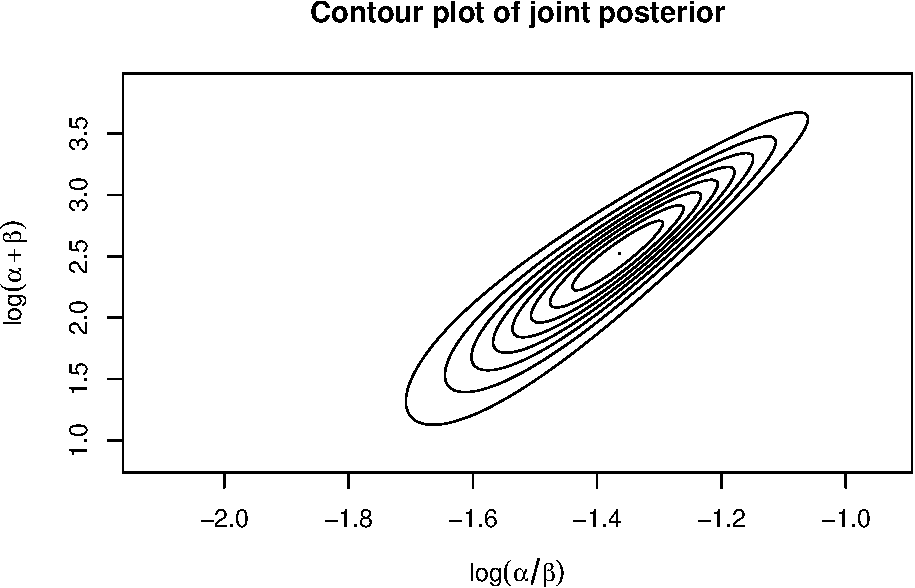
\includegraphics{Untitled_files/figure-latex/unnamed-chunk-19-1.pdf}

Draw samples \((\alpha^{s}, \beta^{s})\) from \(p(\alpha,\beta|y)\)
(finally!). Here we repeat the procedure used in section 3.(v) of the
book replication document.

\begin{Shaded}
\begin{Highlighting}[]
\NormalTok{samps           <-}\StringTok{  }\DecValTok{1000}
\CommentTok{#Integrate (sum) over all beta to get the marginal of alpha}
\NormalTok{v1.dens         <-}\StringTok{  }\KeywordTok{apply}\NormalTok{(post.dens ,}\DecValTok{1}\NormalTok{, sum)}
\NormalTok{s.v1            <-}\StringTok{  }\KeywordTok{sample}\NormalTok{(v1, samps, }\DataTypeTok{replace=}\OtherTok{TRUE}\NormalTok{, }\DataTypeTok{prob =}\NormalTok{ v1.dens)}

\CommentTok{# Select the colum of the joint density corresponding to a specific value of v1 (p(v2|v1))}
\NormalTok{cond.v2         <-}\StringTok{  }\ControlFlowTok{function}\NormalTok{(x) }
\NormalTok{\{}
\NormalTok{  post.dens[}\KeywordTok{which}\NormalTok{(v1 }\OperatorTok{==}\StringTok{ }\NormalTok{s.v1[x]),]}
\NormalTok{\}}
\CommentTok{# Sample a value of v2 according the the conditional probatility above}
\NormalTok{s.v2            <-}\StringTok{  }\KeywordTok{sapply}\NormalTok{(}\DecValTok{1}\OperatorTok{:}\NormalTok{samps,}\ControlFlowTok{function}\NormalTok{(x) }\KeywordTok{sample}\NormalTok{(v2,}\DecValTok{1}\NormalTok{,}\DataTypeTok{replace=}\OtherTok{TRUE}\NormalTok{,}\DataTypeTok{prob=}\KeywordTok{cond.v2}\NormalTok{(x)))}

\CommentTok{# Add a uniform random jitter centered at zero with with equal to the grid spacing. }
\CommentTok{# This will make the simulation draws more continuous. Plot the sampled values.  }
\NormalTok{grid.v1         <-}\StringTok{  }\NormalTok{v1[}\DecValTok{2}\NormalTok{] }\OperatorTok{-}\StringTok{ }\NormalTok{v1[}\DecValTok{1}\NormalTok{]}
\NormalTok{grid.v2         <-}\StringTok{  }\NormalTok{v2[}\DecValTok{2}\NormalTok{] }\OperatorTok{-}\StringTok{ }\NormalTok{v2[}\DecValTok{1}\NormalTok{]}
\NormalTok{s.v2            <-}\StringTok{  }\NormalTok{s.v2 }\OperatorTok{+}\StringTok{ }\KeywordTok{runif}\NormalTok{(}\KeywordTok{length}\NormalTok{(s.v2),}\OperatorTok{-}\NormalTok{grid.v2}\OperatorTok{/}\DecValTok{2}\NormalTok{,grid.v2}\OperatorTok{/}\DecValTok{2}\NormalTok{)}
\NormalTok{s.v1            <-}\StringTok{  }\NormalTok{s.v1 }\OperatorTok{+}\StringTok{ }\KeywordTok{runif}\NormalTok{(}\KeywordTok{length}\NormalTok{(s.v1),}\OperatorTok{-}\NormalTok{grid.v1}\OperatorTok{/}\DecValTok{2}\NormalTok{,grid.v1}\OperatorTok{/}\DecValTok{2}\NormalTok{)}
\KeywordTok{plot}\NormalTok{(s.v1, s.v2, }
     \DataTypeTok{xlab=}\KeywordTok{expression}\NormalTok{( }\KeywordTok{log}\NormalTok{(alpha}\OperatorTok{/}\NormalTok{beta)}\OperatorTok{^}\NormalTok{s ), }
     \DataTypeTok{ylab=}\KeywordTok{expression}\NormalTok{( }\KeywordTok{log}\NormalTok{(alpha}\OperatorTok{+}\NormalTok{beta)}\OperatorTok{^}\NormalTok{s ), }
     \DataTypeTok{xlim=}\KeywordTok{c}\NormalTok{( }\KeywordTok{min}\NormalTok{(v1) , }\KeywordTok{max}\NormalTok{(v1) ) , }
     \DataTypeTok{ylim=}\KeywordTok{c}\NormalTok{( }\KeywordTok{min}\NormalTok{(v2) , }\KeywordTok{max}\NormalTok{(v2) ), }
     \DataTypeTok{main=}\StringTok{"Scatter Plot of Sample Draws of log(alpha/beta) and log(alpha+beta)"}\NormalTok{)}
\end{Highlighting}
\end{Shaded}

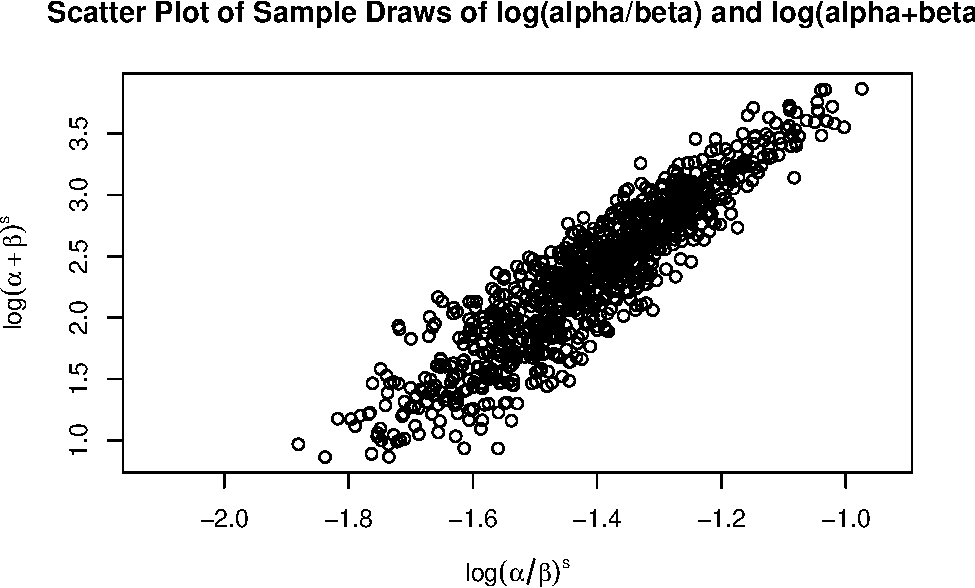
\includegraphics{Untitled_files/figure-latex/unnamed-chunk-20-1.pdf}

By applying the inverse of the transformation we recover the marginal
distribution of the original hyper-parameters.

\begin{Shaded}
\begin{Highlighting}[]
\NormalTok{s.beta          <-}\StringTok{  }\KeywordTok{exp}\NormalTok{( s.v2 ) }\OperatorTok{/}\StringTok{ }\NormalTok{( }\KeywordTok{exp}\NormalTok{(s.v1)}\OperatorTok{+}\DecValTok{1}\NormalTok{ )}
\NormalTok{s.alpha         <-}\StringTok{  }\KeywordTok{exp}\NormalTok{( s.v2 }\OperatorTok{+}\StringTok{ }\NormalTok{s.v1 ) }\OperatorTok{/}\StringTok{ }\NormalTok{( }\KeywordTok{exp}\NormalTok{(s.v1)}\OperatorTok{+}\DecValTok{1}\NormalTok{ )  }
\end{Highlighting}
\end{Shaded}

\subsubsection{5.13c}\label{c-3}

For each draw of \(\phi^{s}\), draw a sample of \(\theta\) from
\(p(\theta|\phi^{s},y)\)

\begin{Shaded}
\begin{Highlighting}[]
\NormalTok{theta.dist      <-}\StringTok{  }\KeywordTok{sapply}\NormalTok{(}\DecValTok{1}\OperatorTok{:}\DecValTok{10}\NormalTok{, }
                           \ControlFlowTok{function}\NormalTok{(x) }
                             \KeywordTok{rbeta}\NormalTok{(}\DecValTok{1000}\NormalTok{, s.alpha}\OperatorTok{+}\NormalTok{y[x], s.beta }\OperatorTok{+}\StringTok{ }\NormalTok{n[x] }\OperatorTok{-}\StringTok{ }\NormalTok{y[x])}
\NormalTok{                           )}
\NormalTok{theta.dist      <-}\StringTok{  }\KeywordTok{apply}\NormalTok{(theta.dist,}\DecValTok{2}\NormalTok{,sort)}
\KeywordTok{plot}\NormalTok{(}\DecValTok{0}\OperatorTok{:}\DecValTok{600}\OperatorTok{/}\DecValTok{1000}\NormalTok{, }\DecValTok{0}\OperatorTok{:}\DecValTok{600}\OperatorTok{/}\DecValTok{1000}\NormalTok{,  }
     \DataTypeTok{type=}\StringTok{"l"}\NormalTok{, }
     \DataTypeTok{xlab=}\StringTok{"Observed rate"}\NormalTok{,}
     \DataTypeTok{ylab=}\StringTok{"95% CI and median of posterior"}\NormalTok{)}

\NormalTok{jitter.x        <-}\StringTok{  }\NormalTok{y}\OperatorTok{/}\NormalTok{n }\OperatorTok{+}\StringTok{ }\KeywordTok{runif}\NormalTok{(}\KeywordTok{length}\NormalTok{(y),}\OperatorTok{-}\FloatTok{0.01}\NormalTok{,}\FloatTok{0.01}\NormalTok{)}
\KeywordTok{points}\NormalTok{(jitter.x, theta.dist[}\DecValTok{500}\NormalTok{,])}
\KeywordTok{segments}\NormalTok{(jitter.x,theta.dist[}\DecValTok{25}\NormalTok{,], jitter.x,theta.dist[}\DecValTok{975}\NormalTok{,] )}
\KeywordTok{title}\NormalTok{(}\DataTypeTok{main=}\StringTok{"Posterior Distribution of Bike rates for all 10 streets"}\NormalTok{)}
\end{Highlighting}
\end{Shaded}

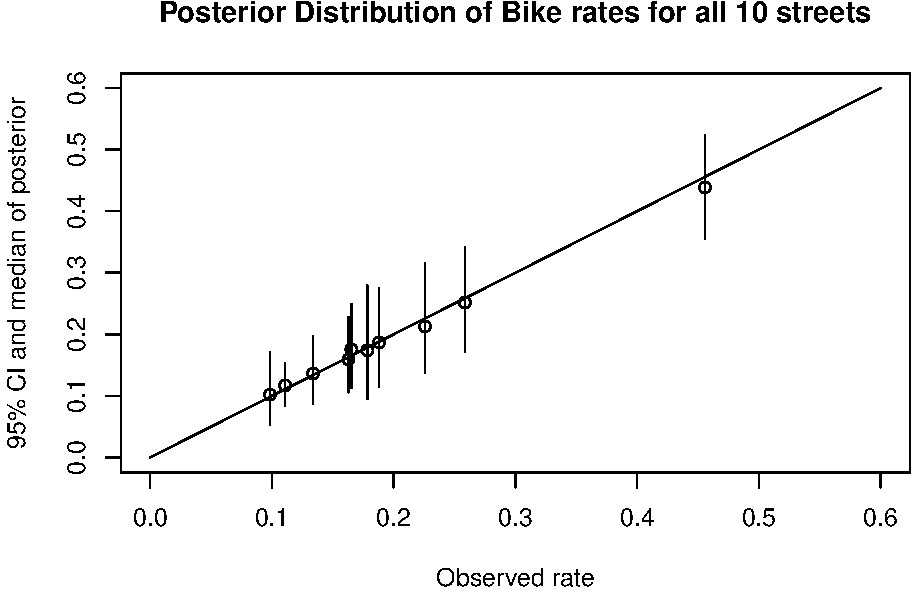
\includegraphics{Untitled_files/figure-latex/unnamed-chunk-22-1.pdf}

The estimated proportions are almost the same as the raw proportions (no
shrinkage).

\subsubsection{5.13d}\label{d-2}

We generate 1000 draws from a \(Beta(\alpha^{s},\beta^{s})\) where the
parameters come from the draws obtained above:

\begin{Shaded}
\begin{Highlighting}[]
\NormalTok{s.theta         <-}\StringTok{ }\KeywordTok{rbeta}\NormalTok{(}\DecValTok{1000}\NormalTok{, }\DataTypeTok{shape1 =}\NormalTok{s.alpha , }\DataTypeTok{shape2 =}\NormalTok{ s.beta)   }
\NormalTok{CI.num          <-}\StringTok{ }\KeywordTok{round}\NormalTok{(s.theta[}\KeywordTok{order}\NormalTok{(s.theta)][}\KeywordTok{c}\NormalTok{(}\DecValTok{25}\NormalTok{,}\DecValTok{975}\NormalTok{)],}\DecValTok{2}\NormalTok{)}
\NormalTok{CI.str          <-}\StringTok{ }\KeywordTok{paste}\NormalTok{(}\StringTok{"("}\NormalTok{ , CI.num[}\DecValTok{1}\NormalTok{] , }\StringTok{","}\NormalTok{ , CI.num[}\DecValTok{2}\NormalTok{] , }\StringTok{")"}\NormalTok{)}
\end{Highlighting}
\end{Shaded}

The posterior interval for \(\hat{\theta} = ( 0.01 , 0.48 )\)

\subsubsection{5.13e}\label{e}

If a new street is opening with 100 vehicles per day. The posterior
interval predicts with 95\% confidence that between 1 and 48. This CI is
not so informative as it covers almost all the possible observed bike
rates.

\subsubsection{5.13f}\label{f}

The beta assumption might not have been so reasonable as the posterior
estimates did not show much shrinkage.

\subsection{5.14}\label{section-3}

\subsubsection{5.14a}\label{a-5}

Set up a model in which the total number of vehicles observed at each
location \(j\) follows a Poisson distribution with parameter
\(\theta_{j}\), the `true' rate of traffic per hour at the location.
Assign a gamma population distribution for the parameters \(\theta_{j}\)
and a non-informative hyper-prior distribution. Write down the joint
posterior distribution.

Now we have that \(n_{j} \sim Poi(\lambda =\theta_{j})\) and
\(\theta_{j} \sim Gamma(\alpha)\). And the joint posterior is:

\[
\begin{aligned}
p(\theta,\alpha,\beta|y) &\propto p(\alpha, \beta) \times p(\theta|\alpha, \beta) \times p(y|\theta,\alpha, \beta) \nonumber \\ 
p(\theta,\alpha,\beta|y) &\propto 1\times \prod_{j=1}^{10}Gamma(\theta_{j} | \alpha, \beta) \times \prod_{j=1}^{10}Poisson(y_{j}|\theta_{j}) \nonumber \\
&= \prod_{j=1}^{10}\frac{\beta^{\alpha}}{\Gamma(\alpha)}\theta_{j}^{\alpha-1}exp(-\beta \theta) \times \frac{\theta_{j}^{y_{i}}exp(-\theta_{j})}{!y_{j}} \nonumber \\
&\propto \frac{\beta^{n\alpha}}{\Gamma(\alpha)^{n}}exp(-\sum \theta_{j}( 1 + \beta )) \prod_{j=1}^{10} \theta_{j}^{\alpha + y_{j}-1} \label{bic.joint.post2}
\end{aligned}
\]

\subsubsection{5.14b}\label{b-4}

Then compute the marginal posterior of \(\theta\), conditional on
\(\alpha, \beta\). For the gamma-poisson case we have that given the
hyper-parameters, each \(\theta_{j}\) has a posterior distribution
\(Gamma(\alpha + n_{j}, \beta +1)\). Assuming exchangeability:

\[
\begin{aligned}
p(\theta|\alpha,\beta,y) &\propto \prod_{j=1}^{10}Gamma(\theta_{j} | \alpha +y_{j}, \beta+1) \nonumber \\
&\propto \prod_{j=1}^{10}Gamma(\theta_{j} | \alpha +y_{j}, \beta+1) \nonumber \\
&\propto \prod_{j=1}^{10} \theta_{j}^{\alpha + y_{j} -1}exp(-(\beta+1) \theta_{j})
\label{bic.cond.post.theta2}
\end{aligned}
\]

Now we compute the posterior marginal of \((\alpha,\beta)\). Given that
we do have a closed form solution in step 2, we compute the ratio of
(\textbackslash{}ref\{bic.joint.post2\}) and
(\textbackslash{}ref\{bic.cond.post.theta2\}). \[
\begin{aligned}
p(\alpha,\beta|y) &\propto \frac{\beta^{n\alpha}}{\Gamma(\alpha)^{n}} \prod_{i=1}^{n}\frac{\Gamma(\alpha+y_{i})}{(\beta + 1)^{\alpha+y_{i}}}
\label{bic.marg.post.phi}
\end{aligned}
\]

Centering our grid around the methods of moments estimates for
\((\alpha_{0}, \beta_{0})\):

\[
\begin{aligned}
\hat{\mu}     &= 116  = \frac{\hat{\alpha_{0}}}{\hat{\beta_{0}}}\\
\hat{\sigma^2} &= 5141.7777778 = \frac{\hat{\alpha_{0}}}{\hat{\beta_{0}}^2}
\end{aligned}
\]

Solving for \((\hat{\alpha_{0}},\hat{\beta_{0}})\):

\begin{Shaded}
\begin{Highlighting}[]
\CommentTok{#Here 'x' represents alpha and beta}
\NormalTok{dslnex          <-}\StringTok{ }\ControlFlowTok{function}\NormalTok{(x) \{}
\NormalTok{    z           <-}\StringTok{ }\KeywordTok{numeric}\NormalTok{(}\DecValTok{2}\NormalTok{)}
\NormalTok{    z[}\DecValTok{1}\NormalTok{]        <-}\StringTok{ }\NormalTok{x[}\DecValTok{1}\NormalTok{]}\OperatorTok{/}\NormalTok{(x[}\DecValTok{2}\NormalTok{]) }\OperatorTok{-}\StringTok{ }\KeywordTok{mean}\NormalTok{(n)}
\NormalTok{    z[}\DecValTok{2}\NormalTok{]        <-}\StringTok{ }\NormalTok{x[}\DecValTok{1}\NormalTok{]}\OperatorTok{/}\NormalTok{(x[}\DecValTok{2}\NormalTok{]}\OperatorTok{^}\DecValTok{2}\NormalTok{) }\OperatorTok{-}\StringTok{ }\KeywordTok{sd}\NormalTok{(n)}\OperatorTok{^}\DecValTok{2}
\NormalTok{    z}
\NormalTok{\}}

\NormalTok{sol1            <-}\StringTok{ }\KeywordTok{nleqslv}\NormalTok{(}\KeywordTok{c}\NormalTok{(}\DecValTok{1}\NormalTok{,}\DecValTok{1}\NormalTok{), dslnex) }
\NormalTok{res1            <-}\StringTok{ }\KeywordTok{paste}\NormalTok{(}\StringTok{"("}\NormalTok{,}\KeywordTok{round}\NormalTok{(sol1}\OperatorTok{$}\NormalTok{x[}\DecValTok{1}\NormalTok{],}\DecValTok{1}\NormalTok{), }\StringTok{","}\NormalTok{, }\KeywordTok{round}\NormalTok{(sol1}\OperatorTok{$}\NormalTok{x[}\DecValTok{2}\NormalTok{],}\DecValTok{2}\NormalTok{), }\StringTok{")"}\NormalTok{,}\DataTypeTok{sep=}\StringTok{""}\NormalTok{)}
\end{Highlighting}
\end{Shaded}

We get: \((\hat{\alpha_{0}},\hat{\beta_{0}}) = (2.6,0.02)\).

We center the grid (approximately) around that initial estimate and
expand the grid to cover up to a factor of 4 of each parameter. The
result is plotted in the following figure:

\begin{Shaded}
\begin{Highlighting}[]
\NormalTok{bic.marg.post.phi <-}\StringTok{   }\ControlFlowTok{function}\NormalTok{(alpha, beta) \{}
\NormalTok{  log.post          <-}\StringTok{  }\DecValTok{0}
  \CommentTok{#notice the censoring in n}
  \ControlFlowTok{for}\NormalTok{ (i }\ControlFlowTok{in} \DecValTok{1}\OperatorTok{:}\KeywordTok{length}\NormalTok{(n)) }
\NormalTok{  \{}
    \ControlFlowTok{if}\NormalTok{ (n[i] }\OperatorTok{>}\StringTok{ }\DecValTok{100}\NormalTok{) n[i]  <-}\StringTok{  }\DecValTok{100}
\NormalTok{    log.post        <-}\StringTok{  }\NormalTok{log.post }\OperatorTok{+}\StringTok{ }\KeywordTok{log}\NormalTok{(}\KeywordTok{gamma}\NormalTok{( alpha}\OperatorTok{+}\NormalTok{n[i] )) }\OperatorTok{-}\StringTok{ }\NormalTok{(alpha}\OperatorTok{+}\NormalTok{n[i])}\OperatorTok{*}\KeywordTok{log}\NormalTok{((beta }\OperatorTok{+}\StringTok{ }\DecValTok{1}\NormalTok{))}
\NormalTok{  \}}
  \CommentTok{# The hyper prior is defined below}
  \KeywordTok{log}\NormalTok{(}\KeywordTok{bic.hyper.prior2}\NormalTok{(alpha,beta)) }\OperatorTok{+}\StringTok{ }
\StringTok{    }\NormalTok{log.post }\OperatorTok{+}\StringTok{ }\NormalTok{(}\KeywordTok{length}\NormalTok{(n)}\OperatorTok{*}\NormalTok{alpha)}\OperatorTok{*}\KeywordTok{log}\NormalTok{(beta) }\OperatorTok{-}\StringTok{ }
\StringTok{    }\KeywordTok{length}\NormalTok{(n)}\OperatorTok{*}\KeywordTok{log}\NormalTok{(}\KeywordTok{gamma}\NormalTok{(alpha))}
\NormalTok{\}}

\NormalTok{bic.hyper.prior2 <-}\StringTok{  }\ControlFlowTok{function}\NormalTok{(alpha,beta) \{}
  \DecValTok{1}
\NormalTok{\}}


\NormalTok{alpha           <-}\StringTok{  }\KeywordTok{seq}\NormalTok{(sol1}\OperatorTok{$}\NormalTok{x[}\DecValTok{1}\NormalTok{]}\OperatorTok{/}\FloatTok{1.5}\NormalTok{,sol1}\OperatorTok{$}\NormalTok{x[}\DecValTok{1}\NormalTok{]}\OperatorTok{*}\FloatTok{1.5}\NormalTok{,}\DataTypeTok{length.out =}\DecValTok{151}\NormalTok{)}
\NormalTok{beta            <-}\StringTok{  }\KeywordTok{seq}\NormalTok{(sol1}\OperatorTok{$}\NormalTok{x[}\DecValTok{2}\NormalTok{]}\OperatorTok{/}\FloatTok{1.5}\NormalTok{,sol1}\OperatorTok{$}\NormalTok{x[}\DecValTok{2}\NormalTok{]}\OperatorTok{*}\FloatTok{1.5}\NormalTok{,}\DataTypeTok{length.out =}\DecValTok{151}\NormalTok{)}

\NormalTok{post.dens       <-}\StringTok{  }\KeywordTok{outer}\NormalTok{(alpha,beta,}\ControlFlowTok{function}\NormalTok{(x1,x2) }\KeywordTok{bic.marg.post.phi}\NormalTok{(x1, x2) )}
\NormalTok{post.dens       <-}\StringTok{  }\KeywordTok{exp}\NormalTok{(post.dens }\OperatorTok{-}\StringTok{ }\KeywordTok{max}\NormalTok{(post.dens))}
\NormalTok{post.dens       <-}\StringTok{  }\NormalTok{post.dens}\OperatorTok{/}\KeywordTok{sum}\NormalTok{(post.dens)}



\NormalTok{contours        <-}\StringTok{ }\KeywordTok{seq}\NormalTok{(}\KeywordTok{min}\NormalTok{(post.dens), }\KeywordTok{max}\NormalTok{(post.dens), }\DataTypeTok{length=}\DecValTok{10}\NormalTok{)}
\KeywordTok{contour}\NormalTok{(alpha, beta, post.dens,}\DataTypeTok{levels=}\NormalTok{contours, }
        \DataTypeTok{xlab=}\KeywordTok{expression}\NormalTok{(alpha), }
        \DataTypeTok{ylab=}\KeywordTok{expression}\NormalTok{(beta), }
        \DataTypeTok{xlim=}\KeywordTok{c}\NormalTok{(}\KeywordTok{min}\NormalTok{(alpha),}\KeywordTok{max}\NormalTok{(alpha)) , }
        \DataTypeTok{ylim=}\KeywordTok{c}\NormalTok{(}\KeywordTok{min}\NormalTok{(beta),}\KeywordTok{max}\NormalTok{(beta)), }
        \DataTypeTok{drawlabels=}\OtherTok{FALSE}\NormalTok{, }
        \DataTypeTok{main=}\StringTok{"Contour plot of joint posterior"}\NormalTok{)}
\end{Highlighting}
\end{Shaded}

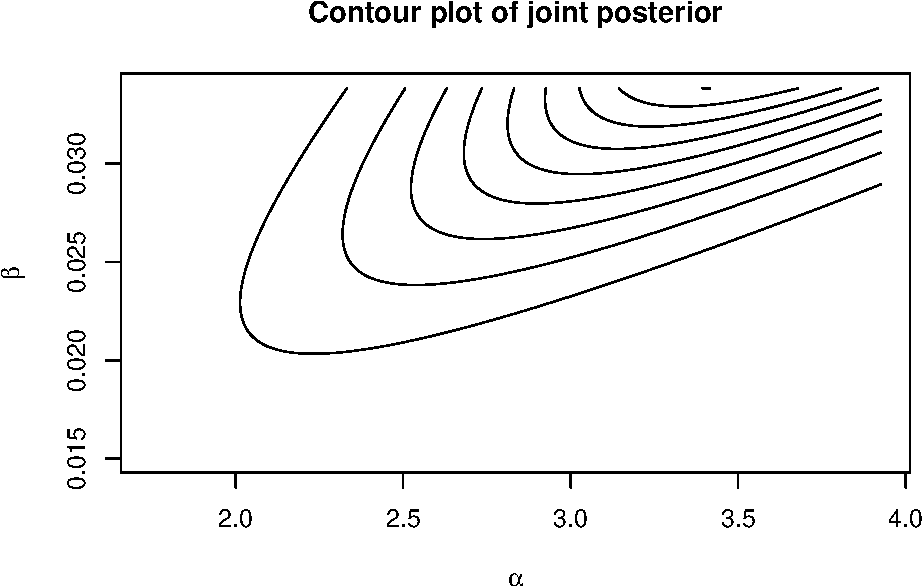
\includegraphics{Untitled_files/figure-latex/unnamed-chunk-25-1.pdf}

Adjust the grid and repeat:

\begin{Shaded}
\begin{Highlighting}[]
\NormalTok{alpha           <-}\StringTok{  }\KeywordTok{seq}\NormalTok{(sol1}\OperatorTok{$}\NormalTok{x[}\DecValTok{1}\NormalTok{]}\OperatorTok{/}\FloatTok{1.5}\NormalTok{,sol1}\OperatorTok{$}\NormalTok{x[}\DecValTok{1}\NormalTok{]}\OperatorTok{*}\DecValTok{12}\NormalTok{,}\DataTypeTok{length.out =}\DecValTok{151}\NormalTok{)}
\NormalTok{beta            <-}\StringTok{  }\KeywordTok{seq}\NormalTok{(sol1}\OperatorTok{$}\NormalTok{x[}\DecValTok{2}\NormalTok{]}\OperatorTok{/}\FloatTok{1.5}\NormalTok{,sol1}\OperatorTok{$}\NormalTok{x[}\DecValTok{2}\NormalTok{]}\OperatorTok{*}\DecValTok{12}\NormalTok{,}\DataTypeTok{length.out =}\DecValTok{151}\NormalTok{)}

\NormalTok{post.dens       <-}\StringTok{  }\KeywordTok{outer}\NormalTok{(alpha,beta,}\ControlFlowTok{function}\NormalTok{(x1,x2) }\KeywordTok{bic.marg.post.phi}\NormalTok{(x1, x2) )}
\NormalTok{post.dens       <-}\StringTok{  }\KeywordTok{exp}\NormalTok{(post.dens }\OperatorTok{-}\StringTok{ }\KeywordTok{max}\NormalTok{(post.dens))}
\NormalTok{post.dens       <-}\StringTok{  }\NormalTok{post.dens}\OperatorTok{/}\KeywordTok{sum}\NormalTok{(post.dens)}

\NormalTok{contours        <-}\StringTok{ }\KeywordTok{seq}\NormalTok{(}\KeywordTok{min}\NormalTok{(post.dens), }\KeywordTok{max}\NormalTok{(post.dens) , }\DataTypeTok{length=}\DecValTok{10}\NormalTok{)}
\KeywordTok{contour}\NormalTok{(alpha, beta, post.dens,}\DataTypeTok{levels=}\NormalTok{contours, }
        \DataTypeTok{xlab=}\KeywordTok{expression}\NormalTok{(alpha), }
        \DataTypeTok{ylab=}\KeywordTok{expression}\NormalTok{(beta), }
        \DataTypeTok{xlim=}\KeywordTok{c}\NormalTok{(}\KeywordTok{min}\NormalTok{(alpha),}\KeywordTok{max}\NormalTok{(alpha)) , }
        \DataTypeTok{ylim=}\KeywordTok{c}\NormalTok{(}\KeywordTok{min}\NormalTok{(beta),}\KeywordTok{max}\NormalTok{(beta)), }
        \DataTypeTok{drawlabels=}\OtherTok{FALSE}\NormalTok{, }
        \DataTypeTok{main=}\StringTok{"Contour plot of joint posterior"}\NormalTok{)}
\end{Highlighting}
\end{Shaded}

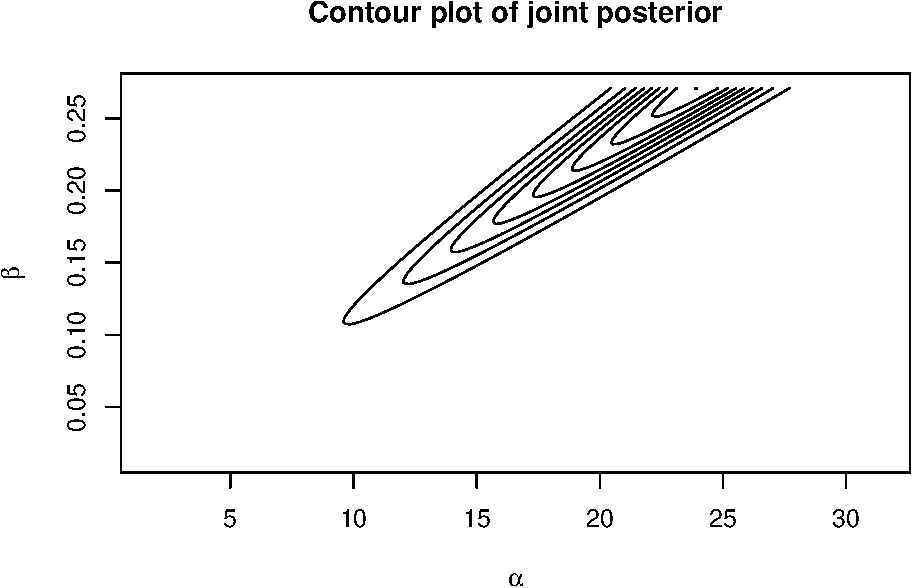
\includegraphics{Untitled_files/figure-latex/unnamed-chunk-26-1.pdf}

Draw samples \((\alpha^{s}, \beta^{s})\) from \(p(\alpha,\beta|y)\).

\begin{Shaded}
\begin{Highlighting}[]
\NormalTok{samps           <-}\StringTok{  }\DecValTok{1000}
\NormalTok{alpha.dens      <-}\StringTok{  }\KeywordTok{apply}\NormalTok{(post.dens ,}\DecValTok{1}\NormalTok{, sum)}
\NormalTok{s.alpha         <-}\StringTok{  }\KeywordTok{sample}\NormalTok{(alpha,samps, }\DataTypeTok{replace=}\OtherTok{TRUE}\NormalTok{, }\DataTypeTok{prob =}\NormalTok{ alpha.dens)}

\CommentTok{#Select the colum of the joint density corresponding to a specific }
\CommentTok{#value of v1 (p(beta|alpha))}
\NormalTok{cond.beta       <-}\StringTok{  }\ControlFlowTok{function}\NormalTok{(x) \{}
\NormalTok{  post.dens[}\KeywordTok{which}\NormalTok{(alpha }\OperatorTok{==}\StringTok{ }\NormalTok{s.alpha[x]),]}
\NormalTok{\}}
\CommentTok{#Sample a value of v2 according the the conditional probatility above}
\NormalTok{s.beta          <-}\StringTok{  }\KeywordTok{sapply}\NormalTok{(}\DecValTok{1}\OperatorTok{:}\NormalTok{samps,}\ControlFlowTok{function}\NormalTok{(x) }
  \KeywordTok{sample}\NormalTok{(beta,}\DecValTok{1}\NormalTok{,}\DataTypeTok{replace=}\OtherTok{TRUE}\NormalTok{,}\DataTypeTok{prob=}\KeywordTok{cond.beta}\NormalTok{(x)))}

\CommentTok{#Add a uniform random jitter centered at zero with with equal to the }
\CommentTok{#grid spacing. This will make the simulation draws more continuous. }
\CommentTok{#Plot the sampled values.  }
\NormalTok{grid.alpha      <-}\StringTok{  }\NormalTok{alpha[}\DecValTok{2}\NormalTok{]}\OperatorTok{-}\NormalTok{alpha[}\DecValTok{1}\NormalTok{]}
\NormalTok{grid.beta       <-}\StringTok{  }\NormalTok{beta[}\DecValTok{2}\NormalTok{]}\OperatorTok{-}\NormalTok{beta[}\DecValTok{1}\NormalTok{]}
\NormalTok{s.beta          <-}\StringTok{  }\NormalTok{s.beta }\OperatorTok{+}\StringTok{ }\KeywordTok{runif}\NormalTok{(}\KeywordTok{length}\NormalTok{(s.beta),}\OperatorTok{-}\NormalTok{grid.beta}\OperatorTok{/}\DecValTok{2}\NormalTok{,grid.beta}\OperatorTok{/}\DecValTok{2}\NormalTok{)}
\NormalTok{s.alpha         <-}\StringTok{  }\NormalTok{s.alpha }\OperatorTok{+}\StringTok{ }\KeywordTok{runif}\NormalTok{(}\KeywordTok{length}\NormalTok{(s.alpha),}\OperatorTok{-}\NormalTok{grid.alpha}\OperatorTok{/}\DecValTok{2}\NormalTok{,grid.alpha}\OperatorTok{/}\DecValTok{2}\NormalTok{)}
\KeywordTok{plot}\NormalTok{(s.alpha, s.beta, }
     \DataTypeTok{xlab=}\KeywordTok{expression}\NormalTok{(alpha), }
     \DataTypeTok{ylab=}\KeywordTok{expression}\NormalTok{(beta), }
     \DataTypeTok{xlim=}\KeywordTok{c}\NormalTok{(}\KeywordTok{min}\NormalTok{(alpha),}\KeywordTok{max}\NormalTok{(alpha)) , }
     \DataTypeTok{ylim=}\KeywordTok{c}\NormalTok{(}\KeywordTok{min}\NormalTok{(beta),}\KeywordTok{max}\NormalTok{(beta)), }
     \DataTypeTok{main=}\StringTok{"Scatter Plot of Sample Draws of alpha and beta"}\NormalTok{)}
\end{Highlighting}
\end{Shaded}

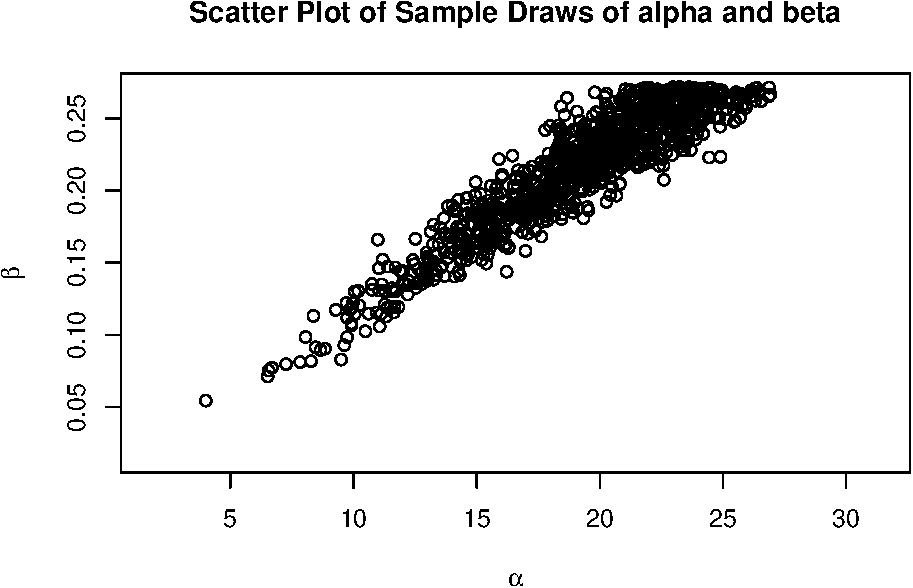
\includegraphics{Untitled_files/figure-latex/unnamed-chunk-27-1.pdf}

\textbf{Note:} regardless of how much I change the range of \(\alpha\)
and \(\beta\) I don't seem to cover the whole graph.

\subsubsection{5.14c}\label{c-4}

Given the previous result we can say that the posterior is not
integrable.

\subsubsection{5.14d}\label{d-3}

I don't know how to alter it such that it becomes integrable.

\subsection{\texorpdfstring{5.15 \textbf{{[}NEW{]}}
Meta-analysis}{5.15 {[}NEW{]} Meta-analysis}}\label{new-meta-analysis}


\end{document}
